%%
%% Copyright 2007, 2008, 2009 Elsevier Ltd
%%
%% This file is part of the 'Elsarticle Bundle'.
%% ---------------------------------------------
%%
%% It may be distributed under the conditions of the LaTeX Project Public
%% License, either version 1.2 of this license or (at your option) any
%% later version.  The latest version of this license is in
%%    http://www.latex-project.org/lppl.txt
%% and version 1.2 or later is part of all distributions of LaTeX
%% version 1999/12/01 or later.
%%
%% The list of all files belonging to the 'Elsarticle Bundle' is
%% given in the file `manifest.txt'.
%%

%% Template article for Elsevier's document class `elsarticle'
%% with numbered style bibliographic references
%% SP 2008/03/01
%%
%%
%%
%% $Id: elsarticle-template-num.tex 4 2009-10-24 08:22:58Z rishi $
%%
%%
\documentclass[preprint,12pt,3p]{elsarticle}


%% Use the option review to obtain double line spacing
%% \documentclass[preprint,review,12pt]{elsarticle}

%% Use the options 1p,twocolumn; 3p; 3p,twocolumn; 5p; or 5p,twocolumn
%% for a journal layout:
%% \documentclass[final,1p,times]{elsarticle}
%% \documentclass[final,1p,times,twocolumn]{elsarticle}
%% \documentclass[final,3p,times]{elsarticle}
%% \documentclass[final,3p,times,twocolumn]{elsarticle}
%% \documentclass[final,5p,times]{elsarticle}
%% \documentclass[final,5p,times,twocolumn]{elsarticle}

%% if you use PostScript figures in your article
%% use the graphics package for simple commands
%% \usepackage{graphics}
%% or use the graphicx package for more complicated commands
%% \usepackage{graphicx}
%% or use the epsfig package if you prefer to use the old commands
%% \usepackage{epsfig}

%% The amssymb package provides various useful mathematical symbols
\usepackage{amssymb}
%% The amsthm package provides extended theorem environments
%% \usepackage{amsthm}

%% The lineno packages adds line numbers. Start line numbering with
%% \begin{linenumbers}, end it with \end{linenumbers}. Or switch it on
%% for the whole article with \linenumbers after \end{frontmatter}.
%% \usepackage{lineno}

%% natbib.sty is loaded by default. However, natbib options can be
%% provided with \biboptions{...} command. Following options are
%% valid:

%%   round  -  round parentheses are used (default)
%%   square -  square brackets are used   [option]
%%   curly  -  curly braces are used      {option}
%%   angle  -  angle brackets are used    <option>
%%   semicolon  -  multiple citations separated by semi-colon
%%   colon  - same as semicolon, an earlier confusion
%%   comma  -  separated by comma
%%   numbers-  selects numerical citations
%%   super  -  numerical citations as superscripts
%%   sort   -  sorts multiple citations according to order in ref. list
%%   sort&compress   -  like sort, but also compresses numerical citations
%%   compress - compresses without sorting
%%
%% \biboptions{comma,round}

% \biboptions{}


\usepackage[utf8]{inputenc}

\usepackage{graphicx}
\usepackage{color}
\graphicspath{ {pics/} }
\usepackage{subfig}

\journal{The International Journal of Digital Forensics and Incident Response}

\begin{document}

\begin{frontmatter}

\title{How to Detect Cryptocurrency Miners? By Traffic Forensics!}

\author[label1]{Vladimír Veselý\corref{cor1}}
\cortext[cor1]{Corresponding author}
\ead{veselyv@fit.vutbr.cz}
\ead[url]{www.fit.vutbr.cz/~veselyv}

\author[label1]{Martin Žádník}
\ead{izadnik@fit.vutbr.cz}
\ead[url]{www.fit.vutbr.cz/~izadnik}

\address[label1]{Brno University of Technology, Božetěchova 2, Brno 612 66, Czech Republic}

\begin{abstract}
Cryptocurrencies set a new trend for a financial interaction between people. In order to successfully meet this use-case, cryptocurrencies combine various advanced information technologies (e.g., blockchain as a replicated database, asymmetrical ciphers and hashes guaranteeing integrity properties, peer-to-peer networking providing fault-tolerant service). Mining process not only introduces new cryptocurrency units, but it has become a business how to generate revenue in real life.
This paper aims at different approaches how to detect cryptocurrency mining within corporate networks (where it should not be present). Mining activity is often a sign of malware presence or unauthorized exploitation of company resources. The article provides an in-depth overview of pooled mining process including deployment and operational details. Two detection methods and their implementations are available for network administrators, law enforcement agents and the general public interested in cryptocurrency mining forensics.    
\end{abstract}

\begin{keyword}
%% keywords here, in the form: keyword \sep keyword
Bitcoin \sep cryptocurrency \sep mining pool \sep mining server \sep Stratum protocol \sep GetBlockTemplate protocol \sep GetWork protocol
%% MSC codes here, in the form: \MSC code \sep code
%% or \MSC[2008] code \sep code (2000 is the default)
\end{keyword}

\end{frontmatter}

%%
%% Start line numbering here if you want
%%
% \linenumbers

%% ===========================================================

\section{Introduction}
\label{sec1}

%% Kontext kryptomen
The motivation behind cryptocurrency is to introduce an alternative currency that is not controlled by a government (e.g., the central bank). Trustworthiness of such electronic cryptocurrency lies in the utilization of cryptographical algorithms to verify transactions and fair emission of new units into circulation. Dark web marketplaces utilize cryptocurrencies for their: a) nearly instant and free-of-charge payments; b) easily obtainable and changeable addresses; c) hard to trace transactions (thanks to their peer-to-peer nature). Several studies \cite{RAESSI15}, \cite{GRINBERG14}, \cite{JOHNSON14} investigate Bitcoin as the key component of any digital black marketplace because cryptocurrencies generally allow criminals to circumvent law enforcement agencies (LEAs) and regulators. 

%% Kontext Bitcoinu a minitutorial nad pojmy
Of all cryptocurrencies, Bitcoin \cite{BTCPAPER}, \cite{BTCORG} had become popular when it gained momentum at the end of 2013 after its exchange price skyrocketed. The current (at the August 2018) total number of Bitcoins (approx. 17.1 million) accounts for more than 139 billion USD \cite{BTCCAP}. Bitcoin is a peer-to-peer network with the distributed infrastructure of users and miners. A miner verifies ongoing transactions for a reward (either transaction fee or newly emitted Bitcoins). The reward is paid to the first miner who proves transaction by spending its computation power on this process. Other proof-of-work\footnote{In case of  \textit{proof-of-work} mining, the probability of finding a new block is directly proportional to a computational power invested in mining. While for \textit{proof-of-stake} mining, the probability is directly proportional to a number of units owned by a miner.} cryptocurrencies also adopted the same mining concept. Anyone can join the solo mining process but the probability of earning a reward is low and the risk of wasted computational power without any profit too high. Therefore, miners form so-called mining pools. When the pool earns a reward, it is distributed by the pool operator among miners according to their contribution. 

Apart from alternatives to Bitcoin (e.g., Litecoin, Ethereum, generally referred as \textit{(alt)coins}), the cryptocurrency universe also contains \textit{tokens}. Tokens (comparing to coins) represent digital asset or utility that leverages another's coin blockchain for being accounted. New tokens are generally not mined but distributed by their authors/owners. In the frame of this paper, we will focus only on the mining process behind coins and refer to them as "cryptocurrencies" interchangeably.

%% Proc se zabyvame detekci tezaru
Any organization should be aware of running mining software on its hardware in its network due to at least two reasons: a) the mining activity is often caused by malware, therefore, the mining activity is an indicator of a compromise; b) the energy (e.g., electricity, cooling, CPU and GPU power) spent on mining is paid by the hosting organization, but the recipient of the reward is a malicious actor. This survey \cite{ali2015bitcoin} speaks about various types of cryptocurrency malware dedicated to undercover mining on devices, desktops, and servers but also platforms like webcams, smartphones or network attached storages. Universities \cite{THEGUARDIAN-STUDENT} or technological centers \cite{CCN-STUDENT}, \cite{INDEPENDENT-BANSCIENTIST} are typical examples of energy exploitation because they offer free computational resources (i.e., servers, network) to academics, researchers and students. Nevertheless, it is possible to start a mining operation in any organization including subsidized accommodation for Czech members of parliament \cite{AKTUALNE-PIRAT}.  

The malicious actor might exploit these assets in such environment resulting in the increased energy bill, depleted resources, endangered work processes and other users. For instance, Bitcoin mining has a severe impact on electricity comparable to the energy consumption of Ireland \cite{ENERGY14} in 2014. Another report \cite{de2018bitcoin} provides a more in-depth analysis of how to estimate Bitcoin's hunger for energy concluding that it may reach 7.67 gigawatts (comparable with Austria) during 2018. The reader must take into account that Bitcoin mining is just a tip of the iceberg, which consists of all proof-of-work cryptocurrencies.

%% Jak na detekci jdeme
In this paper, we focus on the detection of devices participating in the mining pools. Cryptocurrency mining is the only option how users may obtain freshly minted currency units. Moreover, mining is still the prevailing form of how to earn cryptorcurrencies with the existing equipment.

We propose two approaches how to detect cryptocurrency miners in the network:

\begin{itemize}
    \item The first approach is based on a mix of passive and active traffic monitoring. The passive monitoring is based on the analysis of IP flow records, while the active monitoring is based on probing. The detection method as a whole slowly learns a list of mining servers which subsequently reduces the need for the active monitoring. Since anyone can set up own mining pool or even mining server, the resulting list of publicly known mining servers cannot be considered complete. However, it may be employed as a baseline for miner detection by any network operator. 
    \item The second approach can be described as a catalog of mining pools. We have created a publicly available web application that stores metadata about existing mining pools. Any user may query our system to check whether a given FQDN\footnote{Fully qualified domain name (FQDN) is complete host identification within a Domain Name System (DNS) tree hierarchy.}, IP address or port number is a part of known pool configuration.
\end{itemize}  

The contribution of this article involves: a) an overview of the current cryptocurrency mining technology; b) two detection methods to detect network traffic related with cryptocurrency mining; c) open-access data samples; and d) publicly available service cataloging mining servers.

%% Struktura clanku
The rest of the paper is organized as follows. Section \ref{sec2} informs about related work on cryptocurrency mining. Section \ref{sec3} brings details about currently used mining architecture and involved protocols. Section \ref{sec4} describes passive/active traffic monitoring (the first approach how to detect miners), which also includes its validation and verification. Section \ref{sec5} explains the implementation and operation of the mining server catalog (the second approach). The article is summarized in Section \ref{sec6}, which also outlines our future work. 

%% ===========================================================

\section{Related Work}
\label{sec2}
This section summarizes knowledge from the selected articles relevant to cryptocurrency mining. We try to motivate miners detection in a frame of known cryptocurrency issues and research of others. 

%% Offloading Bitcoin 101 na jine clanky
We consider Courtois et al. \cite{courtois2013unreasonable} work as a great introductory source explaining Bitcoin mining. Despite focusing on Bitcoin mining process improvement, authors provide theoretical background explaining bindings between employed cryptography and cryptocurrency mining. Moreover, this work and other ones mentioned in this section allow us to skip thorough the cryptographic description of the mining process. Instead of it, we will focus only on protocols and messages exchanged between miner and pool.

%% Cim se take zabyvame
Kroll et al. \cite{kroll2013economics} and Lawenberg et. al \cite{lewenberg2015bitcoin} provide an economical point of view on Bitcoin mining. They try to model the mining process as the game-theory problem. Eyal and Sirer \cite{eyal2014majority} discuss Bitcoin security and mining incentive-compatibility. All of these articles introduce interesting attacks that might disrupt any cryptocurrency mining process. We will briefly mention mining protocol "flaws" that may be used to identify miner and connect its identity with a real person.

%% Motivace za kryptomenami
Several studies \cite{juels2016ring}, \cite{hampton2015ransomware}, \cite{ali2015zombiecoin}, \cite{kharraz2015cutting} mention ways and means how cryptocurrencies are being employed in monetizing and as a platform for unlawful activities. Examples include ransomware attacks, botnet command and control operations, private keys thefts, spam advertisements, pay-per-click or pay-per-install scams and others. Our research complements these studies by targeting the illicit mining of cryptocurrencies.

%% Detekce mineru jako dukaz existence malwaru
Huang et al. \cite{huang2014botcoin} provide a comprehensive study of cryptocurrency mining malware. Authors developed methods, which correlate the mining bot with its mining pool. Moreover, authors were able to estimate the number of infected devices, generated revenue and duration of botnet infection. We consider this paper as a great stimulation for our work because it shows how successful discovery of miners can be crucial not only for proper network operation but also for significant reduction of botnets contagions. There is a connection between (unintentional) cryptocurrency mining and exploitation of resources.

D’Herdt \cite{SANSREPORT} analyzed captured traffic samples and suggested to look for well-known ports and IP addresses of mining servers. Besides that, he derived that the communication of miners with mining server is sparse but often cyclic between 30-100s. Although it is possible to capture all the network traffic even on a high-speed link~\cite{hanic} so that the raw network data can be analyzed, it is a resource-expensive way of network monitoring from a long-term perspective. 

%%%%%%%%%%%%%%%%%%%%%%%%%%%%%%%%%%%%%%%%%%%%%%%%%%%%%%%%%%%%%%%%%%%
%a it is certainly not , the current best practise of network monitoring is usually based on passive monitoring of some  this renders the enormous amount of data infeasible for a long-term storage and quite complicated for online analysis.
%%%%%%%%%%%%%%%%%%%%%%%%%%%%%%%%%%%%%%%%%%%%%%%%%%%%%%%%%%%%%%%%%%%
 
Therefore, various meta-data collecting approaches are utilized, among others IP flow monitoring represented by several generations of NetFlow protocols~\cite{RFC3954} and IPFIX~\cite{RFC7011} is widely deployed. The intrinsic characteristic of flow monitoring is a loss of information in comparison with the full packet capture. The flow data analysis is, therefore, less reliable than the packet analysis itself. Nevertheless, flow analysis has found many applications such as network monitoring, application classification, host profiling, accounting and billing \cite{flowapplicationsurvey}.

The research in flow analysis has come up with simplistic as well as complex approaches ranging from statistic methods to machine learning (ML) approaches. As an example, Hofstede et al \cite{sshcompromise} propose a simple statistical method based on the same number of packets per flow in multiple flows to detect attacker trying to brute-force SSH server. More complex methods have been proposed to detect anomalies, e.g., Silveira at al \cite{astute} proposes a complex statistic model to detect strong correlations in simultaneous flow volume changes.

To the best of our knowledge, there has been no work focusing on detection of cryptocurrency miners utilizing flow data.
However, from the perspective of methodology, the closest to our work are methods based on supervised machine learning such as \cite{mlflow}. The authors of \cite{mlflow} select descriptive features that should be extracted from the flow data, prepare an annotated data-set and train a classification model which is used to recognize specific events in the flow data. 

Due to the inherent loss of information in case of flow monitoring and due to the heuristic nature of the analysis methods, there are often false positive results. If the number of false positives is very low, then the heuristic can be deployed. Otherwise, administrators start to ignore the analysis results after several false positives due to a loss of trust in the method.
We address the issue of false positives by combining the results of passive detection and active probing. Such an approach has not been investigated in the previous research.

%%%%%%%%%%%%%%%%%%%%%%%%%%%%%%%%%%%%%%%%%%%%%%%%%%%%%%%%%%%%%%%%%%%
%% diskutovat vyhody naseho pristupu kombinace passive a aktiv
%Various optimizations have been proposed to simplify flow measurement either by focusing on a large flows such as %in~\cite{estan2003new,mori2004identifying} or by estimating characteristics from sampled traffic %directly~\cite{duffield2001charging}.
%\textcolor{red}{doplnit related work za pasivni detekci, napr. rick hofstede, detekci skype apod.}
%%%%%%%%%%%%%%%%%%%%%%%%%%%%%%%%%%%%%%%%%%%%%%%%%%%%%%%%%%%%%%%%%%%


%% ===========================================================

\section{Mining Background}
\label{sec3}
This section provides a theoretical background (mostly based on Bitcoin use-case). However, explanation of the whole mining process for all cryptocurrencies is far beyond the scope of this article. Hence, only parts relevant to the miner detection are captured. The first subsection lays out the basic theory for any cryptocurrency operation. The second subsection familiarizes the reader with the state-of-the-art of cryptocurrency mining software and hardware. The third subsection provides a deeper description of existing mining protocols.

\subsection{Theory}
\label{subsec31}
\textit{Transaction} encapsulates transfer of cryptocurrency units between parties, where a single transaction may contain multiple inputs and also outputs. To prevent fake or malicious transaction (e.g., double spending problem), a given user needs to validate the transaction history. Hence, transactions are chained together, where outputs of the previous transaction serve as inputs of the next transaction. Transactions are grouped into \textit{blocks}, which vouches for the validity of contained transaction with timestamps and cryptographic hashes. Blocks are periodically recorded into public ledger dubbed as \textit{blockchain}. Blocks are bound together in blockchain as a unidirectional list, where each item (i.e., block) has the pointer to its predecessor. The inception of cryptocurrency is done by starting its history with the first \textit{genesis block}. Blocks are formed and their content verified by \textit{miners}, who compete between themselves in the process (so-called \textit{mining}) of appending new blocks to the blockchain. The winning miner earns reward in the form of newly minted coins (called \textit{coinbase transaction}) as an incentive to participate on cryptocurrency peer-to-peer network operation. The winner is the miner, which would successfully solve the certain cryptographic task (e.g., compute a hash with certain properties from given inputs and nonces) of variable \textit{difficulty} (which acts as a feedback mechanism guaranteeing deterministic time of block creation). Miners are grouped in \textit{pools} in order to increase their chance of successful mining and thus to cash the reward.

\subsection{Hardware and Software}
\label{subsec32}
A wide range of different mining hardware/software exist that is mostly differentiated by an employed hashing algorithm and \textit{hashrate} (i.e., computational performance in a number of hashes per second, abbreviated as hash/s). Depending on a given cryptocurrency, the user chooses the appropriate combination of hardware and software that impacts mining operation. Mining hardware capabilities pose an upper-bound limit for a maximum available hashrate. Nevertheless, the choice of mining software may optimize and automatize the mining operation. To generalize it, successful establishment of cryptocurrency mining consists of several steps.

\begin{enumerate}
    \item Select cryptocurrency - It is important to decide which cryptocurrency to mine if the miner speculates on the future price. Hence, it is necessary to take into account: a) trend of exchange price; b) cryptocurrency viability; c) possible increase of mining difficulty; and d) ever-changing total hashrate of the peer-to-peer network. There is no business perspective to mine cryptocurrencies if overall expenses exceed potential income. Due to the very volatile exchange rates between cryptocurrencies and fiat money, the risks are high.
    \item Choose a pool - Participation in the pool (compared to solo mining) offers a more predictable generation of revenue, which is proportional to work done by a miner. It is important to choose a stable pool (in terms of Internet connectivity and denial-of-service protection) with trustworthy pool operator (who will not embezzle earnings or submitted shares for own profit). Available strategies of how are miners rewarded (e.g., Pay Per Share, Pay Per Last N Shares, Shared Maximum PPS, Capped Maximum PPS With Recent Backpay) also affects the selection of the mining pool. Comparison of the most popular mining pools is available at following website \cite{COMPAREPOOL}.
    \item Assemble mining rig - Overall power consumption of the mining rig goes hand to hand with its hashrate performance. Any mining rig dissipates heat that needs to be ventilated out. Improper cooling may lead to unnecessary outages or hardware failures that prolong or even challenges return of investment for mining rig cost. Professional mining rigs are out-of-the-box solutions (packed with GPUs or ASIC-based) that contain industrial air-vents producing a lot of noise. All previously mentioned facts can be used as indicators how to locate mining rig in corporate environment physically. 
    \item Configure mining software - Mining is controlled and managed either by official cryptocurrency client or dedicated software. Mining pool suggests to its members mining software for supported cryptocurrencies. Moreover, the pool provides a personalized configuration which helps miners to start quickly and easily their mining operation. Mining software needs a low-bandwidth, but constant connection to the Internet since it periodically exchanges work packages with the server. 
\end{enumerate}

\begin{figure}[ht]
    \centering
    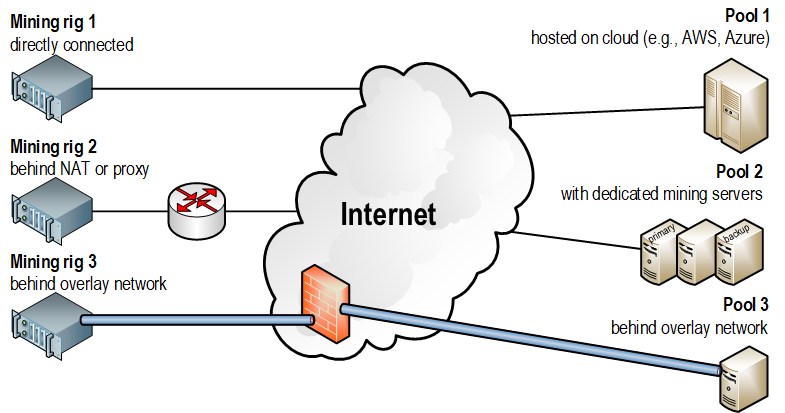
\includegraphics[width=\textwidth]{deploy2.png}
    \caption{Deployment scenarios for miners and pools}
    \label{fig:deploy}
\end{figure}

Figure \ref{fig:deploy} outlines usual deployment scenarios between miners and mining pools. A user may control multiple mining devices (rigs, sometimes also referred to as workers). Each mining device may rotate mining operation (i.e., in a round-robin or fall-back fashion) between multiple pools. Each mining device is connected to a single mining server that belongs to the pool, thou switching to a secondary mining server is quite common in case of the outage of the primary one. The connection between miner and server can be: a) direct without any middle-box (although, it reveals IP address of miner); b) proxied by centralizing communication with mining server via middle-box that may relay or even alter mining protocol data; c) overlayed via VPN\footnote{Virtual Private Network. For more, see https://en.wikipedia.org/wiki/Virtual\_private\_network}, TOR\footnote{The Onion Router. For more, visit https://www.torproject.org/}, I2P\footnote{Invisible Internet Project. For more, check https://geti2p.net/en/} or any similar service.

%% Hardware
Cryptocurrency mining has evolved through the following five generations:

\begin{enumerate}
    \item CPU mining - CPU software mining is the initial way how to verify transaction for the most of young cryptocurrencies when consensus about mining is known, but there is no parallelization or dedicated hardware support yet. Mining on general CPU offers just a fraction of a potential hashrate, but it is easy to develop software for CPU miner. 
    \item GPU mining - Current generations of graphical cards are supercomputers capable of massive parallel computations. GPUs generally have higher hashrate than CPUs, but their effectiveness also depends on employed hashing algorithm (for instance the same GPU card would mine Bitcoins in order of Mhash/s, but Litecoins in khash/s). There is a major difference in hashrate between the two biggest GPU vendors. AMD cards are generally more effective because they have better Arithmetic Logic Unit support comparing to nVidia cards, which are focused on Floating Point Unit operations.  
    \item FPGA mining - Field-programmable gate array chips (FPGAs) have far less power consumption comparing to GPUs, but they do not significantly increase hashrate. FPGAs just like ASICs are available for a limited number of cryptocurrencies because development and manufacturing of these platforms require significant investments and there must be the business reasoning behind.
    \item ASIC mining - Application-specific integrated circuits (ASICs) are the last stage of the mining hardware evolution. ASICs offer the highest mining speeds and the best ratio between hashrate and power consumption. Currently, ASICs availability is limited to doubled SHA-256 \cite{Anonymous2012SHS}, Scrypt \cite{rfc7914} and X11 \cite{DASHX11} hashing algorithms (and accompanied cryptocurrencies). However, ASICs pose a threat to the stability of any cryptocurrency system because of uneven distribution of hashrate, where the minority of ASICs users usually represent the most powerful mining group that may lead to successful 51\% attack \cite{COINDESK51}. Probably due to the appealing return of investment, the history of ASIC-miner manufacturing has lots of examples of false promises \cite{COINDESK-BFLAB}, \cite{COINDESK-COINTERRA} or even scams \cite{COINDESK-ALPHATECH}, \cite{COINDESK-BLACKARROW}. Moreover, a limited number of companies survived this business clash and (at least Bitcoin) ASIC vendor market is dominated by a single company (Bitmain\footnote{Namely a line of products called Antminers, for more see https://shop.bitmain.com/?lang=en}) with nearly none competition (i.e., Canaan Creative\footnote{Namely a line of products called AvalonMiners, for more see https://canaan.io/shop/}).
    \item Cloud mining - The setup of the successful mining operation requires non-trivial IT skills, appropriate software installation and investments in the hardware. Hence, the entry level for mining is too steep for the majority of the population. Therefore, mining rental service has got more and more popular since 2013. Using this service, the customer buys a mining contract for a limited period. A remote miner is paid with the fixed rent, and the customer receives all coins earned by a miner (thus, speculating for a future price of a selected cryptocurrency). For a duration of mining contract, the customer may even switch the configuration to mine a different cryptocurrency (as long as it uses the same hashing algorithm). Following website \cite{COMPARECLOUD} compares different cloud mining services.
\end{enumerate}

To compare generations between each other (and show their impact on the market), we will use Bitcoin and doubled SHA-256 hashrate as the example illustrated in Table \ref{tab:hardware}. Since mining technology evolves fast, we list average hashrates (based on community shared \cite{BITCOINITMINING}, \cite{BITCOINITNONMINING} user experience) of devices available in the year 2013, which was the last year when all five generations coexisted together in Bitcoin mining ecosystem.

\begin{table}
\centering
\begin{tabular}{|l|c|r|} 
    \hline
    \textbf{Hardware} & \textbf{Generation} & \textbf{Hashrate} \\
    \hline\hline
    Intel i7 Core 3930k & CPU & ~66 Mhash/s \\
    \hline
    AMD Radeon 7970 & GPU & ~710 Mhash/s \\
    \hline
    nVidia GeForce GTX 590 & GPU & ~190 Mhash/s \\
    \hline
    BitForce SHA256 Single & FPGA & ~830 Mhash/s \\
    \hline
    ModMiner Quad & FPGA & ~800 Mhash/s \\
    \hline
    ButterFly Labs Single SC & ASIC & ~30 Ghash/s \\
    \hline
    Avalon1 A3256 Miner & ASIC & ~66 Ghash/s \\
    \hline
\end{tabular}
\caption{A comparison of Bitcoin mining hardware relevant to 2013}
\label{tab:hardware} 
\end{table}

%% Software
According to a chosen cryptocurrency, miner needs to install and configure special software which coordinates mining task between mining hardware and the pool. Mining software responsibility is: a) to communicate with the mining server using mining protocol; and b) to relay mining work package for hardware processing. A plethora of consensus methods exists differentiated mostly by employed hashing algorithms. Following Table \ref{tab:software} summarizes some of the existing mining software supporting GPU mining for a selected number of cryptocurrencies:

\begin{table}
\centering
\begin{tabular}{|c|c|c|}
    \hline
    \textbf{Cryptocurrency} & \textbf{Algorithm} & \textbf{Mining software} \\
    \hline\hline
    Bitcoin & SHA-256d & cgminer \\
     &  & BFGMiner \\
    \hline
    Litecoin & Scrypt & cgminer \\
    Dogecoin &  & BFGMiner \\
    \hline
    Dash & X11 & SGMiner \\
     &  & ccMiner \\
    \hline
    Ethereum & Dagger-Hashimoto & ethminer \\
    Ethereum Classic &  & Claymore's Dual Miner \\
    \hline
    ZCash & Equihash & Silent Army ZCash Miner \\
     &  & Claymore's ZCash Miner \\
    \hline
    Monero & Cryptonight & Wolf Miner \\
     &  & ccMiner \\
    \hline
    Vertcoin & Lyra2RE & SGMiner \\
    \hline
\end{tabular}
\caption{Overview of some mining software}
\label{tab:software} 
\end{table}

%% Vladimir - Pokud by byla vule, tak doplnit zhodnoceni ruznych aktualne dostupnych mining SW
The mining software configuration specifies URL of mining server (including port number), username and password for miner's authentication, hardware-related setup (e.g., preferred GPU kernels, graphical card processor, and memory overclocking). Recommended configuration parameters are always available on pool's website (usually together with a mining guide for beginners, see for example \ref{appendix-sec1}) in order to guarantee a smooth and user-friendly setup of the mining operation.

\subsection{Protocols}
\label{subsec33}
A mining pool and its members are using dedicated protocols to coordinate distribution of mining process. There exist three general mining protocols supported by a majority of cryptocurrencies: 

\begin{itemize}
    \item\textit{GetWork} was the first mining protocol ever. Comparing to its descendants, GetWork is a simple request-response scheme protocol, where server assigns work package and miner blindly conducts mining task. Due to its simplicity, GetWork allows double-spent transactions in the case of corrupt pool operator. GetWork messages with JSON\footnote{JavaScript Object Notation. For more, see https://tools.ietf.org/html/rfc7159} syntax are carried inside  HTTP\footnote{Hypertext Transfer Protocol. For more, visit https://tools.ietf.org/html/rfc7230}. GetWork supports a limited number of protocol extensions using additional HTTP header lines.
    \item\textit{GetBlockTemplate} is official mining protocol developed in the frame of Bitcoin community but also adopted by other cryptocurrencies. GetBlockTemplate was codified in BIP\footnote{Bitcoin Improvement Proposal. See https://github.com/bitcoin/bips/blob/master/bip-0002.mediawiki} 22 \cite{BIP22}. GetBlockTemplate is more decentralized by offloading block creation process onto miners instead of pools. GetBlockTemplate increases potential work package size and reduces mining protocol overhead to support performance delivered by ASIC miners. Moreover, BIP 23 \cite{BIP23} standardizes extensions and ways how to flexible improve GetBlockTemplate without any major protocol redesign or non-conformant HTTP header hacks.
    \item\textit{Stratum} protocol \cite{SLUSHSTRATUM} was prototyped by M. Palatinus, inventor of pooled mining and operator of the oldest Slush pool \cite{SLUSHPOOL}. Stratum development was motivated by a need to remedy design flaws of previous two protocols: a) by removing HTTP as a carrier, which reduces unnecessary protocol overhead; b) by removing long polling feature that posed scalability issue for load balancing of traffic between miner and server; and c) by adding \textit{extranonce} field that allows miner to generate more hashes locally without bothering a mining server for a new batch of work. Stratum is JSON-RPC 2.0 \cite{JSONRPC} compatible protocol that operates directly above TCP.
\end{itemize}

All of these protocols leverage TCP\footnote{Transmission Control Protocol. For more, see https://tools.ietf.org/html/rfc793} as the transport layer protocol. Comparing to official cryptocurrency peer-to-peer clients, mining protocols do not use any "well-known" port number. It depends solely on the preference of mining pool administrator on which ports pool servers accept connections. Hence, port numbers 80, 443, and 25 are often used as a best practice how to bypass firewalls between mining device and its mining server. 

The usual message exchange involves several steps. With the initial message, the miner connects to the mining server and provides authentication credentials. Authentication is necessary because based on credentials, mining pool correlates submitted shares with miner's account and credit earnings. Two types of authentication are common: 

\begin{itemize}
    \item \textit{registration-oriented} - Before establishing the mining operation, the user owning mining rig needs to sign up to the pool and create an account. A part of account administration involves workers (i.e., separate mining devices) setup. Authentication credentials inside mining protocol include username and password.
    \item \textit{registration-less} - Some pools tender their services without any dedicated account registration. In that case, the miner usually provides just cryptocurrency address to inform pool where to send payments. This identifier substitutes username and is enough for authentication. 
\end{itemize}

No matter on authentication type, the username may contain optional suffixes such as worker identifier (in order to distinguish different workers of the same user) or e-mail address (where the user is notified about any problems occurred during mining).

The next step in mining protocol communication is a recurrent assignment of work packages provided by the server. Each work package contains \textit{data}, \textit{target}, and \textit{nonce} (other fields depend on cryptocurrency). A miner tries to find a hash (from combined data and nonce) that meets (i.e., is lower than) a target. Different cryptocurrencies are using distinct hashing algorithms - e.g., SHA-256d for Bitcoin, Scrypt for Litecoin, X11 for Dash. Miner either submits correct solution or restarts mining with different inputs upon receiving a new work package. Miner periodically announces its state to the server.

\begin{figure}[ht]
    \centering
    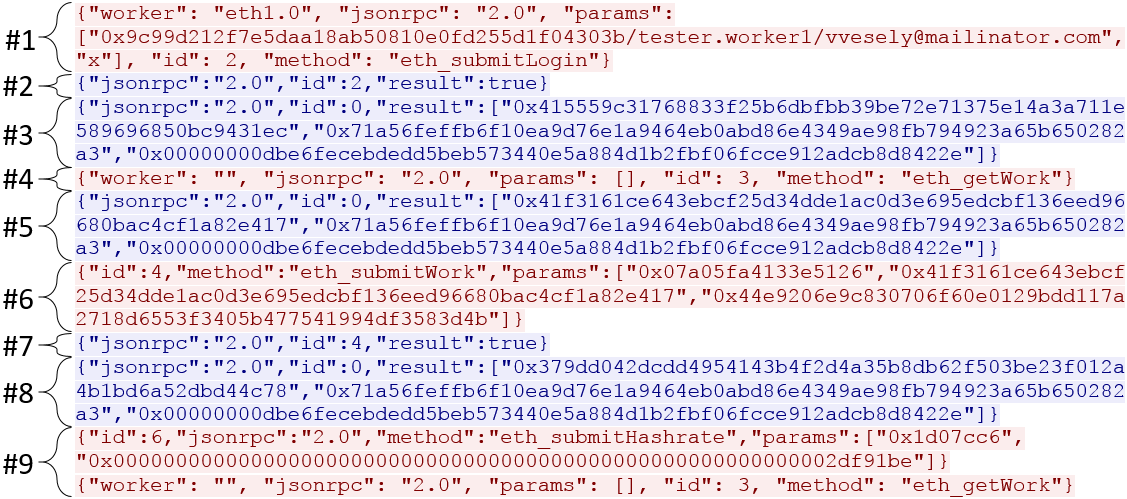
\includegraphics[width=\textwidth]{exchange.png}
    \caption{Example of Stratum protocol message exchange}
    \label{fig:stratum}
\end{figure}

Figure \ref{fig:stratum} illustrates Stratum exchange from mining device to its server (with the red color) and vice versa (the blue color). We can observe the typical confluence of messages. A connection to the pool is initiated with the first message (marked as \#1), where we can see authentication details. The server confirms it with message denoted as \#2. The server sends a work package (\#3) that needs to be computed. Upon proper initialization of mining software, the miner asks for a new work package (\#4), which the mining server gladly provides (\#5). The miner successfully finds the hash and submits (\#6) the complete solution back to the server. The server decides whether the miner's result is valid or not (in the case of \#7, it is valid) and sends a new work package (\#8). The miner starts a new task and meantime periodically updates server about its local computational speed (message marked as \#9) so that server can dynamically adjust the size of subsequent work packages. 
If we focus on the forensic analysis of metadata related to mining protocol, then we can extract:

\begin{itemize}
    \item IP addresses and port numbers - By inspecting IP addresses, we can geolocate both miner and mining server. Together with port numbers, we can account network traffic with NetFlow. Once we have NetFlow records available, we can answer questions such as for how long is mining operation active, how many mining devices are involved, etc.
    \item Pool information - GetWork or GetBlockTemplate protocol extensions may uncover other useful intel such as alternative mining servers including their IP addresses, fully-qualified domain names, and port numbers.
    \item Miner's username - Based on authentication type, username field may contain either nickname or account name of pool user or its cryptocurrency address. This information may be crucial for successful correlation of real-world person and its electronic identity.
    \item Miner's password - Authentication message of any mining protocol includes a password. However, it is seldom used for authorization or any purpose by a pool. The default value of password field for the most of mining software is `x'.
    \item Miner's email - Some pools offer email notifications about the progress of mining operation. In case of any problem such as the miner outage, too many rejected shares or disconnection from the pool, the user is warned by email. The email address may be optionally part of mining protocol message filed, which may help to reveal user's identity.
\end{itemize}

During the implementation phase of our miner's detection methods, we needed relevant data. Hence, we recorded packets exchanged between our testing miner and various pools mining different cryptocurrencies. We offer these Wireshark packet captures as a data-set, which is publicly available at \cite{GITHUB-REPRO} to anyone interested in subsequent research related to mining protocols.

%% ===========================================================

\section{Traffic Monitoring}
\label{sec4}

Active mining clients connect to the pool, ask for a job and deliver the results. Their communication with the mining server offers a possibility for passive detection. If the characteristics of the message exchange are specific enough, we may differentiate miners’ communication from the rest of the traffic. We intend to utilize basic IP flow records (e.g., NetFlow v5) as an input for the passive detection algorithm. This approach is generic and not dependent on the specific capabilities of the monitoring device, which offers more possibilities for broader deployment. On the other hand, we expect a lot of false positives caused by the limited set of input characteristics that are not unique enough. We address the problem by adding the second detection step, where an active connection attempt verifies the identity (whether it belongs to mining pool or not) of the server to which the suspicious client connects to. This active detection is done by probing the potential server with specific JSON message unique to Stratum protocol.
In order to reduce the number of probes, we propose to employ a list of already probed servers. The list stores the probing result (either positive or negative), the destination port number and the timestamp of the probe.
 
\subsection{Design of Cryptocurrency Network Traffic Detector}
\label{subsec41}

We propose to apply a classifier built by a machine learning technique to detect candidate mining communication passively.
But before it is possible to apply machine learning, there must be an annotated data-set that would allow for training and evaluation of the classifier.

\begin{figure}[ht]
    \centering
    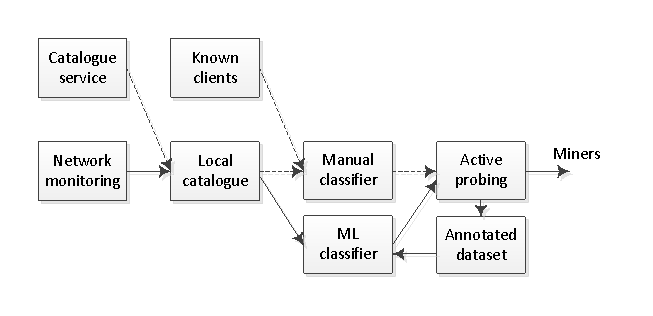
\includegraphics[width=\textwidth]{annotationscheme.pdf}
    \caption{Data annotation process (dashed lines are utilized during the first iteration)}
    \label{fig:scheme}
\end{figure}

Our process of data annotation is based on an iterative approach which allows continuous building of annotated data-set. 
Figure~\ref{fig:scheme} provides the overall view of the process while individual components are elaborated later on.
To start the annotation from scratch, we select features based on the observations of the traffic of local mining clients and the flow data of the well-known mining servers. 
Then we manually construct a simple classifier, which serves as a passive detector, and active probing verifies its results.
Once enough data is annotated, we replace the simple classifier with the classifier trained by machine learning.

%%%%%%%%%%%%%%%%%%%%%%%%%%%%%%%%%%%%%%%%%%%%%%%%%%%%%%%%%%%%%%%%%%%
%should, ideally, correctly classify all miners, i.e. the classifier can trade-off higher number of false positives for zero false negatives.
%%%%%%%%%%%%%%%%%%%%%%%%%%%%%%%%%%%%%%%%%%%%%%%%%%%%%%%%%%%%%%%%%%%

In order to derive the classification features, we analyzed several packet captures collected by observing communication of various mining softwares (e.g., cpuminer) and the traffic belonging to the well-known mining servers.
According to our analysis, we can state that:
\begin{itemize}
\item Mutual communication between a miner and a mining server often lasts for several hours.
\item Packets are generally small, often in the range from 40 to 120 bytes.
\item Most flows contain TCP ACK+PUSH flag set.
\item The destination port is either a well-known port of a different service or not well-known but definitely lower than the source port.
\item Flows are generally long-lasting, often exported before its end.
\item Communication is not disrupted, i.e., most flows do not contain RST flag set.
\end{itemize}

The detection itself starts with feature collection. 
For each triplet (source and destination IP addresses and destination port) following features are collected:
\begin{itemize}
\item an average number of bytes per packet derived from flows belonging to this triplet;
\item an average number of packets per each flow;
\item an average number of packets per minute;
\item duration of a communication;
\item a number of flows;
\item percentage of flows with PUSH+ACK to all flows belonging to this triplet;
\item percentage of flows with RST to all flows belonging to this triplet;
\item percentage of flows with SYN to all flows belonging to this triplet;
\item percentage of flows with FIN to all flows belonging to this triplet;
\item percentage of flows with source port greater than destination port.
\end{itemize}

The triplet and its features are collected in a hash table in a memory.
In order to limit the size of the hash table, triplets are evicted from the table if there is no update for more than a defined number of seconds (we set up this inactive timeout to be one hour). 
However, the passive detection itself is performed periodically, every 60\,s.

In order not to flood the network with active probes right after the start when the list of the probed servers is almost empty (i.e., the list contains well-known mining servers only), the active probing is limited to 100 connections per second. 
As a result, it is not possible to rule out all false positives during the initial period. 
Since we want to report only the true positives, the monitoring scheme reports only verified results by the probe or by the list. 
Therefore false negatives may occur during the initial period.
After the initial period (i.e., after the list is built), the probing becomes less intensive and reach a stable state which is below the limit on the number of probes per second.

The manually-constructed classifier is based on a cumulative score which must overcome a threshold $T$. 
The score is gradually increased by an increment of $1/n$, where $n$ is the number of satisfied conditions listed below:

\begin{itemize}
    \item a number of bytes per packet per each flow is in the range 35 - 80 bytes or 105 - 110 bytes;
    \item a number of packets per each flow is out the range of 5 to 40;
    \item a number of packets per minute is in the range 2 - 8 or 40 - 5300;
    \item duration of communication is greater than 300 s;
    \item percentage of flows with ACK+PUSH to all flows is higher than 90\%;
    \item percentage of flows with SYN to all flows is less than 5\%;
    \item percentage of flows with RST to all flows is less than 1\%;
    \item percentage of flows with FIN to all flows is less than 5\%;
    \item percentage of flows with srcPort greater than dstPort is higher than 90\%.
\end{itemize} 

Unfortunately, it is not the case that each mining client meets all the conditions. Therefore, the detection must take into account communications satisfying only some of conditions. 

%%%%%%%%%%%%%%%%%%%%%%%%%%%%%%%%%%%%%%%%%%%%%%%%%%%%%%%%%%%%%%%%%%%
%Therefore, the score must exceed a threshold $T=<0, 1>$.
%We set up this threshold so that 100\% of positives is accepted.
%Each condition is assigned an equal increment of $1/n$ where $n$ is the number of conditions.
%a weight which favours such conditions that contributes to a final score of the triplet. The weight of each condition $w_{i}$ is calculated as:
%$w_{i} =  (1 - (false_negatives/(false_negatives+true_positives)) ) / n$
%$where $i$ is the order of the feature and $i=1, \ldots , n$.
%In other words 
%%%%%%%%%%%%%%%%%%%%%%%%%%%%%%%%%%%%%%%%%%%%%%%%%%%%%%%%%%%%%%%%%%%

Therefore, the threshold $T$ must be set low enough so that the detector detects the majority of true positives. 
We trade off 100\% true positive rate for the higher number of false positives since we know that the active probing will mitigate the false positives.

The machine learning detector is based on decision tree induction with a particular implementation of J48 in Weka~\cite{weka}.
The decision tree induction recursively selects features and their thresholds to maximize information gain contributed by the selected feature.
This leads to a construction of a sub-optimal but well-performing decision tree.
%Since we only want to show a feasibility of miners detection utilizing machine learning technique we leave finer tuning of the detection as a future work.

No matter whether building manual classifier or training ML-classifier, it is important to bear in mind that any of them may misclassify non-miners for miners. However, the active probe mitigates these false positives. On the other hand, the number of probes must be reasonable (i.e., low enough) not to flood the network.
%The overall detection scheme proceeds with active detection to verify the results of passive detection.

Active detection connects to a mining server pretending to be a regular miner asking for a job. 
If the server replies with an expected answer, then it is very likely that: a) the server is truly mining server; and b) clients connecting to this given server on this particular port are actually miners.
The number of servers to check would be too high without the prior passive detection. 
Even our server running the detection scheme was reported by network monitoring tools as a scanner, while we were developing and testing this approach.
Therefore, it is advisable to limit the number of active probes so that they fly under the radar. 
Based on the size of a network, this number could be 10 to 100 of probes per second.

The probe itself differs based on the mining protocol, where each probe consists of several queries targeting different cryptocurrencies (namely Bitcoin, Monero, Ethereum, Zcash).
The following snippet is an example of a query for Stratum protocol:

\begin{figure}[!h]
    \label{fig:tam}
    \centering
    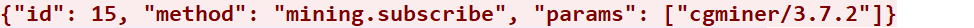
\includegraphics[width=\textwidth]{tam.png}
\end{figure}

%\begin{verbatim}
%{"id ": 1, "method": "mining. subscribe", "params": ["cpuminer/2.4.3"]} 
%\end{verbatim}

The probing itself must run in parallel since it takes time a server to respond or time out. An example of a typical conforming response from a mining server is given below:

\begin{figure}[!h]
    \label{fig:zpet}
    \centering
    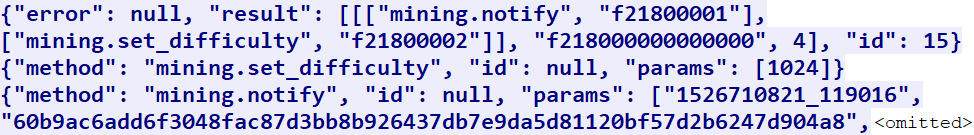
\includegraphics[width=\textwidth]{zpet.png}
\end{figure}

%\begin{verbatim}
%{"error":null,"id":1,"result":[[["mining. set\_difficulty","1"], 
%["mining.notify","1"]] ,"24690500837db5",4]} 
%{"params":[256],"id": null,"method":"mining. set\_difficulty"} 
%{"params":["f3799","3917dd2c463cad43***20000002","180375 ff","5866c43e",
%true], "id": null,"method":"mining.notify"}
%\end{verbatim}

To sum up, the active detection performs following tasks:
\begin{enumerate}
    \item Check whether (\textit{destination IP, destination port})-tuple is on the triplet list of already probed servers.
    \item If \texttt{false}, then probe (\textit{destination IP, destination port})-tuple and store the result in the triplet list together with the current timestamp.
    \item If \texttt{true}, then check the timestamp
    \begin{itemize}
        \item If the timestamp is younger than 7~days, utilize the stored result.
        \item Otherwise, probe the (\textit{destination IP, destination port})-tuple and update the triplet list including a new timestamp.
    \end{itemize}
\end{enumerate}

\subsection{Evaluation}
\label{subsec43}

\subsubsection{Data-sets}
\label{subsubsec431}

The experiments were carried out on data collected in Czech National Research and Educational Network connecting more than 30 organizations (e.g., universities, labs, hospitals) including more than 400 thousand users altogether. 
However, only 3 subnets conforming to 3 large organizations (over 50 thousand users) were considered for training and evaluation of data-set in order to thin the amount of training data and to allow for manual verification of the results. 
The observation points are located on the peering links with internet exchange points or other national networks. Therefore, the communication between entities within the national network is not part of data.
 
\begin{table}[t!]
    \begin{center}
        \begin{tabular}{|l|c|c|c|c|}
        \hline
        &Flows & Packets & Bytes & Interval \\
        \hline
        Train.-eval.  & 16M & 117M & 54G & 2018/02/02 14:00 - 14:15\\
        Real      & 3.6G & 27.8G & 99.5T & 2018/02/09 14:00 - 20:00\\
        \hline
        \end{tabular}
    \caption{Volumes of utilized data-sets.}
    \label{tab:char}
    \end{center}
\end{table}
 
We created an offline data-set consisting of the feature vectors and their classification (i.e., mining/non-mining client). The data-set can be downloaded from the results reproduction page~\cite{GITHUB-REPRO}. This data-set was created by streamwise\footnote{Continuous stream of data rather than fixed length intervals as described in \cite{nemea}} aggregation of IP flow records collected from the backbone described above. The set is annotated utilizing the proposed detection algorithm described above. Therefore, if the triplets are annotated as mining, we know they are true positives (later on referred to as positives only) while the rest (referred to as negatives) are either true negatives (i.e., negative verification by the probe) or potential false negatives (i.e., not verified by the probe).

\subsubsection{Experiments}
\label{subsubsec432}

The feature selection was performed by the analysis of traffic belonging to a known mining client bearing in mind that only basic flow records allow for general deployment. 
The selected features were evaluated on the annotated data-set described in the previous section.
Figure~\ref{fig:histograms} depicts cumulative normalized distribution function (CDF) of the selected features belonging to the triplets as collected by during passive detection. 
Each feature is assigned two functions -- one for samples annotated as miners (positive) and one for samples annotated as other (negative).

\begin{figure}%
    \centering
    \subfloat[bytes per packet]{\label{fig:grafbpp}{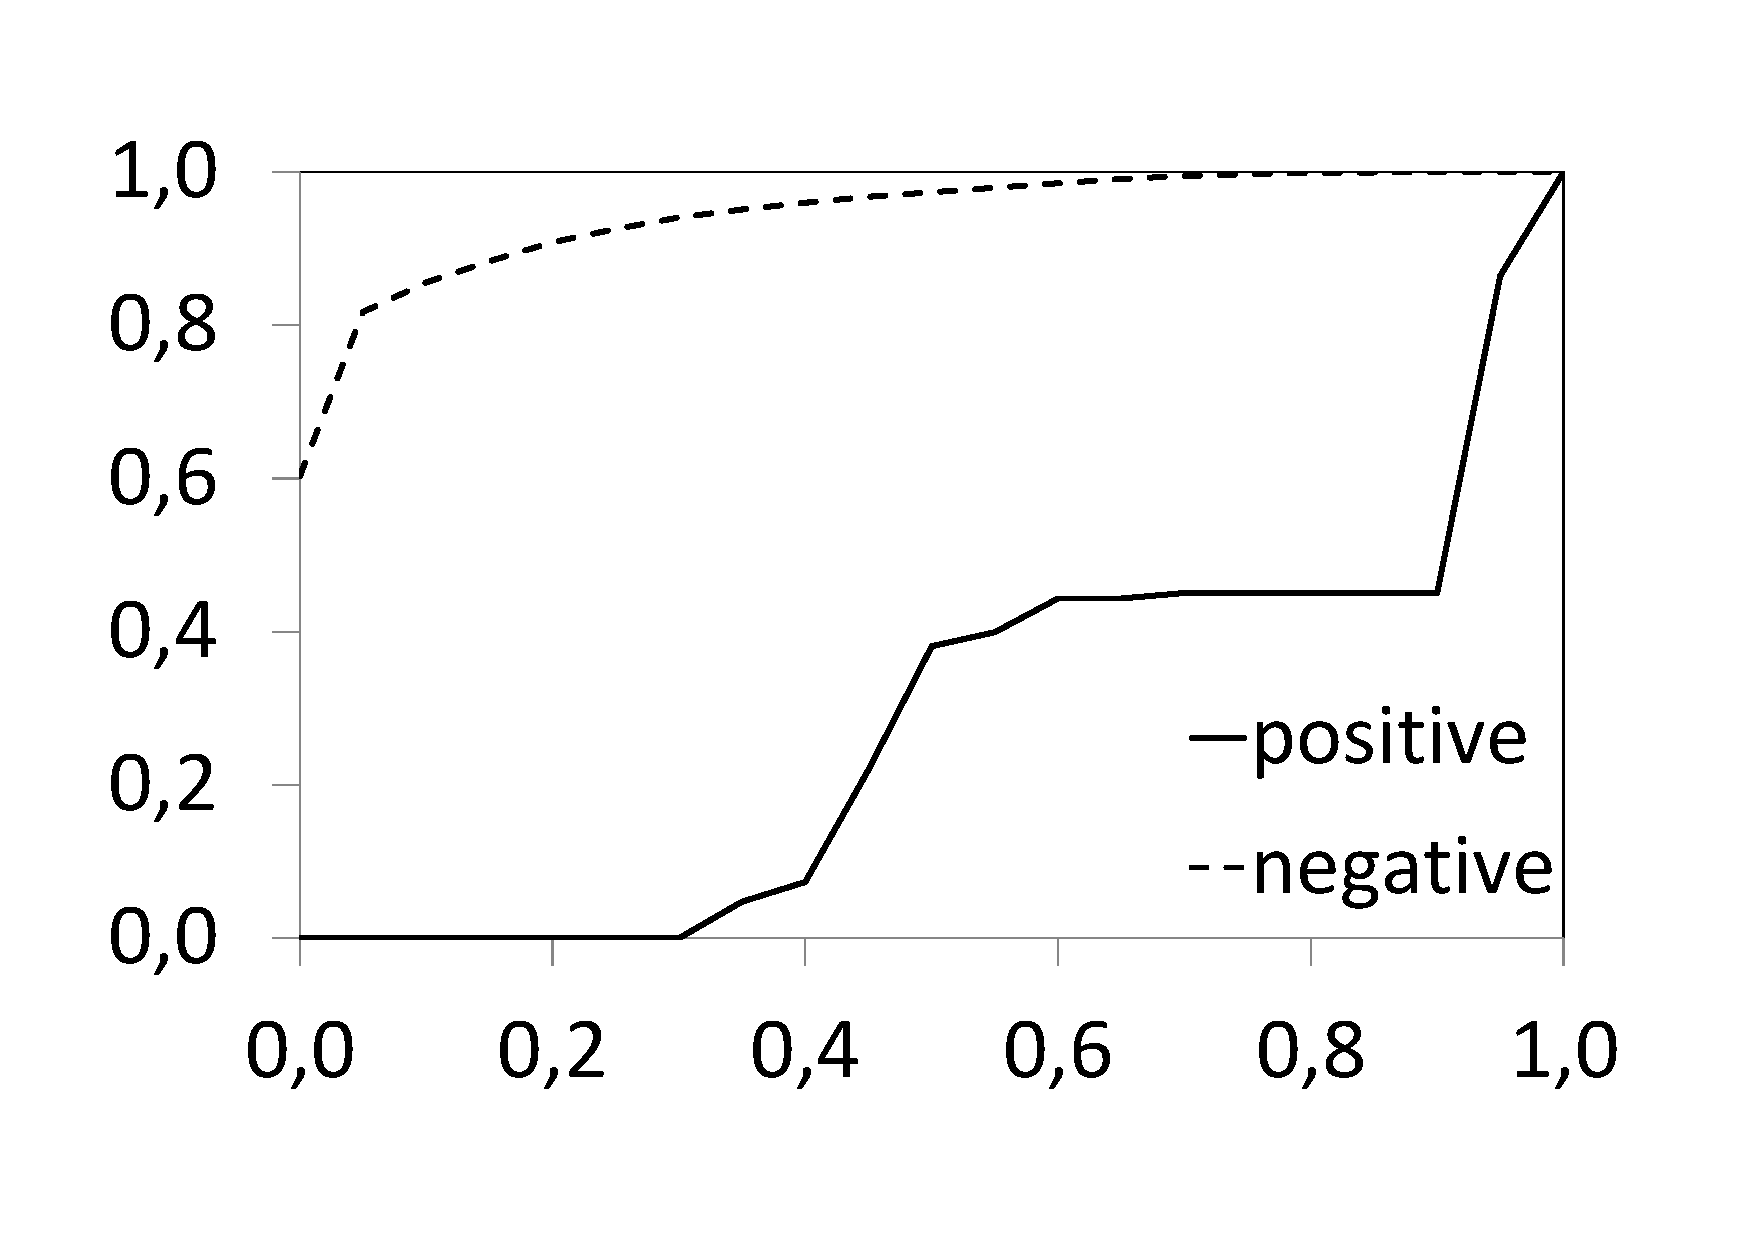
\includegraphics[height=4.1cm]{grafbpp.pdf} }}%
    \qquad
    \subfloat[log$_{10}$ of packets per flow]{\label{fig:graflogppf}{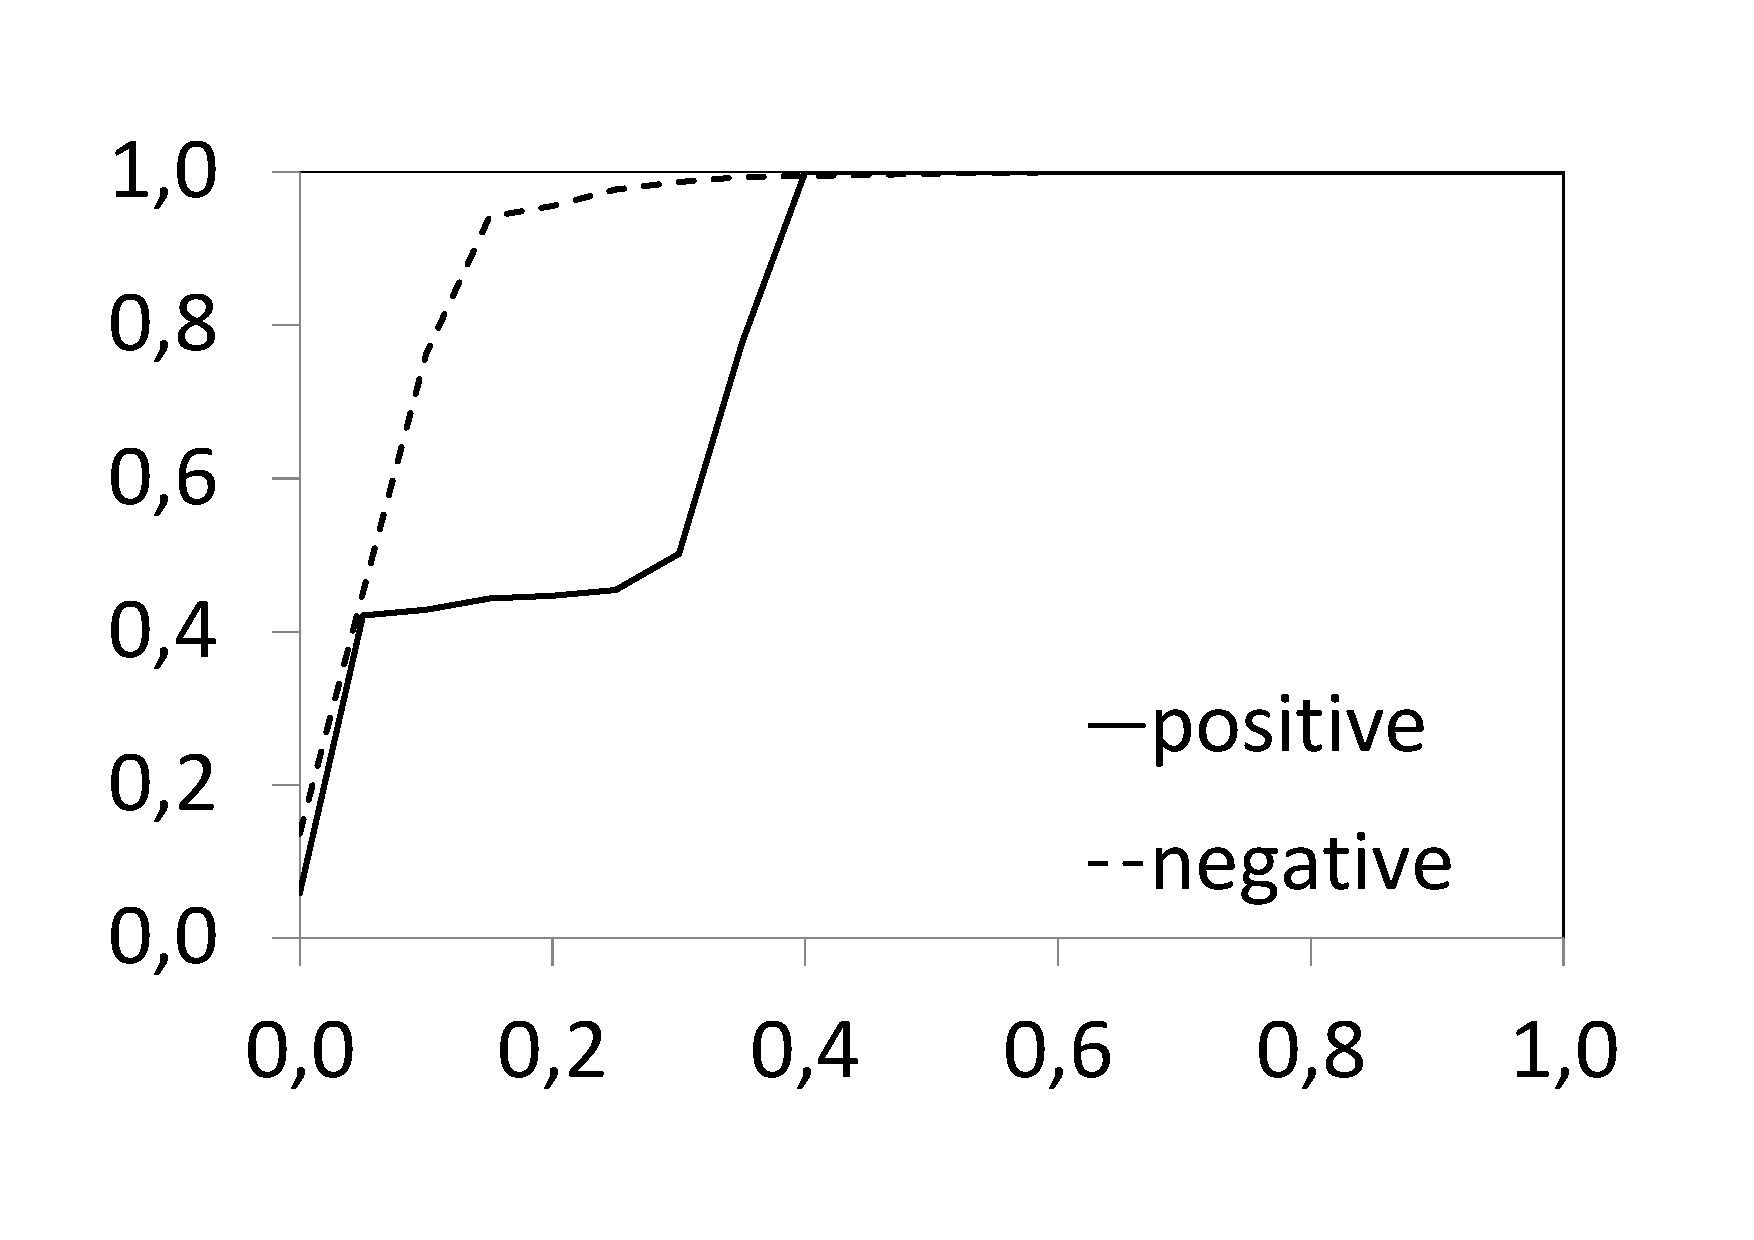
\includegraphics[height=4.1cm]{graflogppf.pdf} }}\\
    \subfloat[log$_{10}$ of packets per minute]{\label{fig:graflogppm}{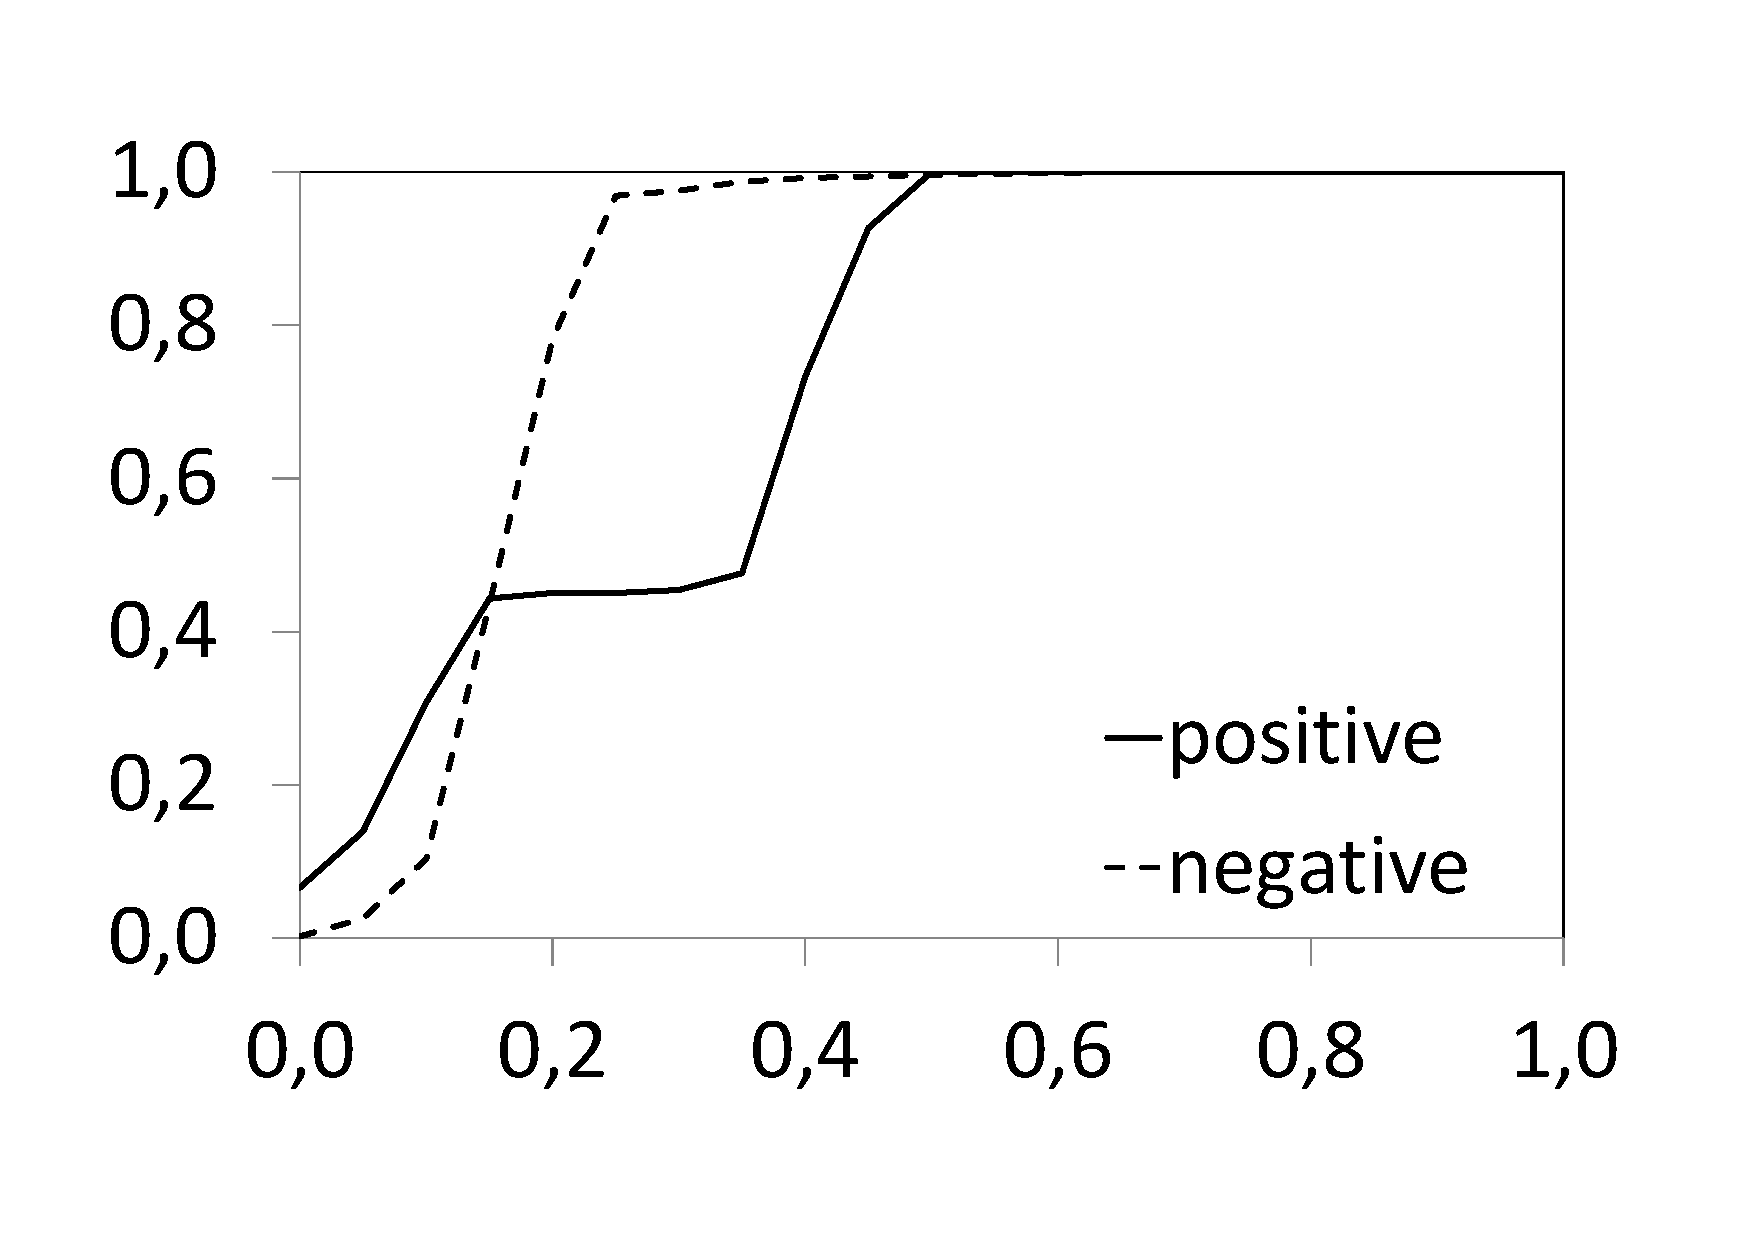
\includegraphics[height=4.1cm]{graflogppm.pdf} }}%
    \qquad
    \subfloat[ACK + PUSH]{\label{fig:grafackpush}{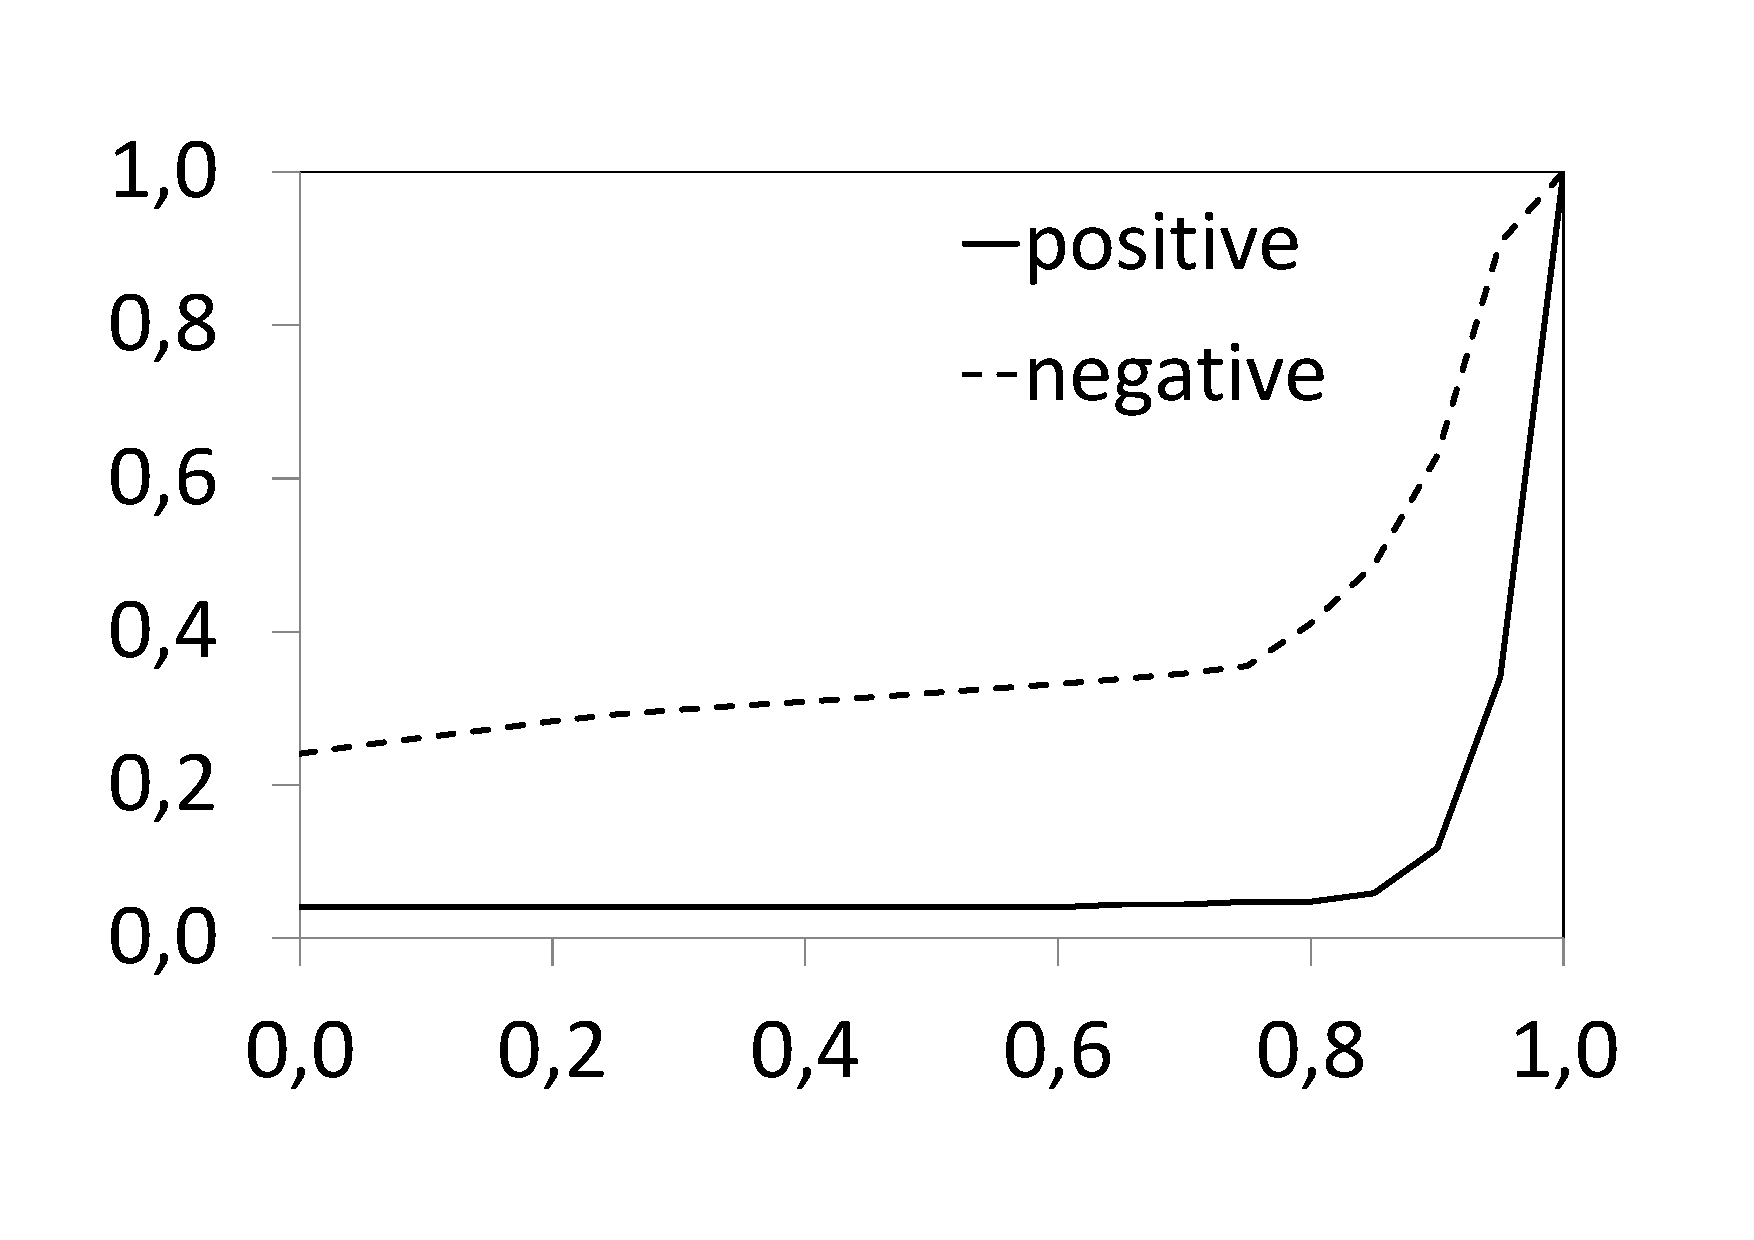
\includegraphics[height=4.1cm]{grafackpush.pdf} }}\\
    \subfloat[SYN / ALL]{\label{fig:grafsyn2all}{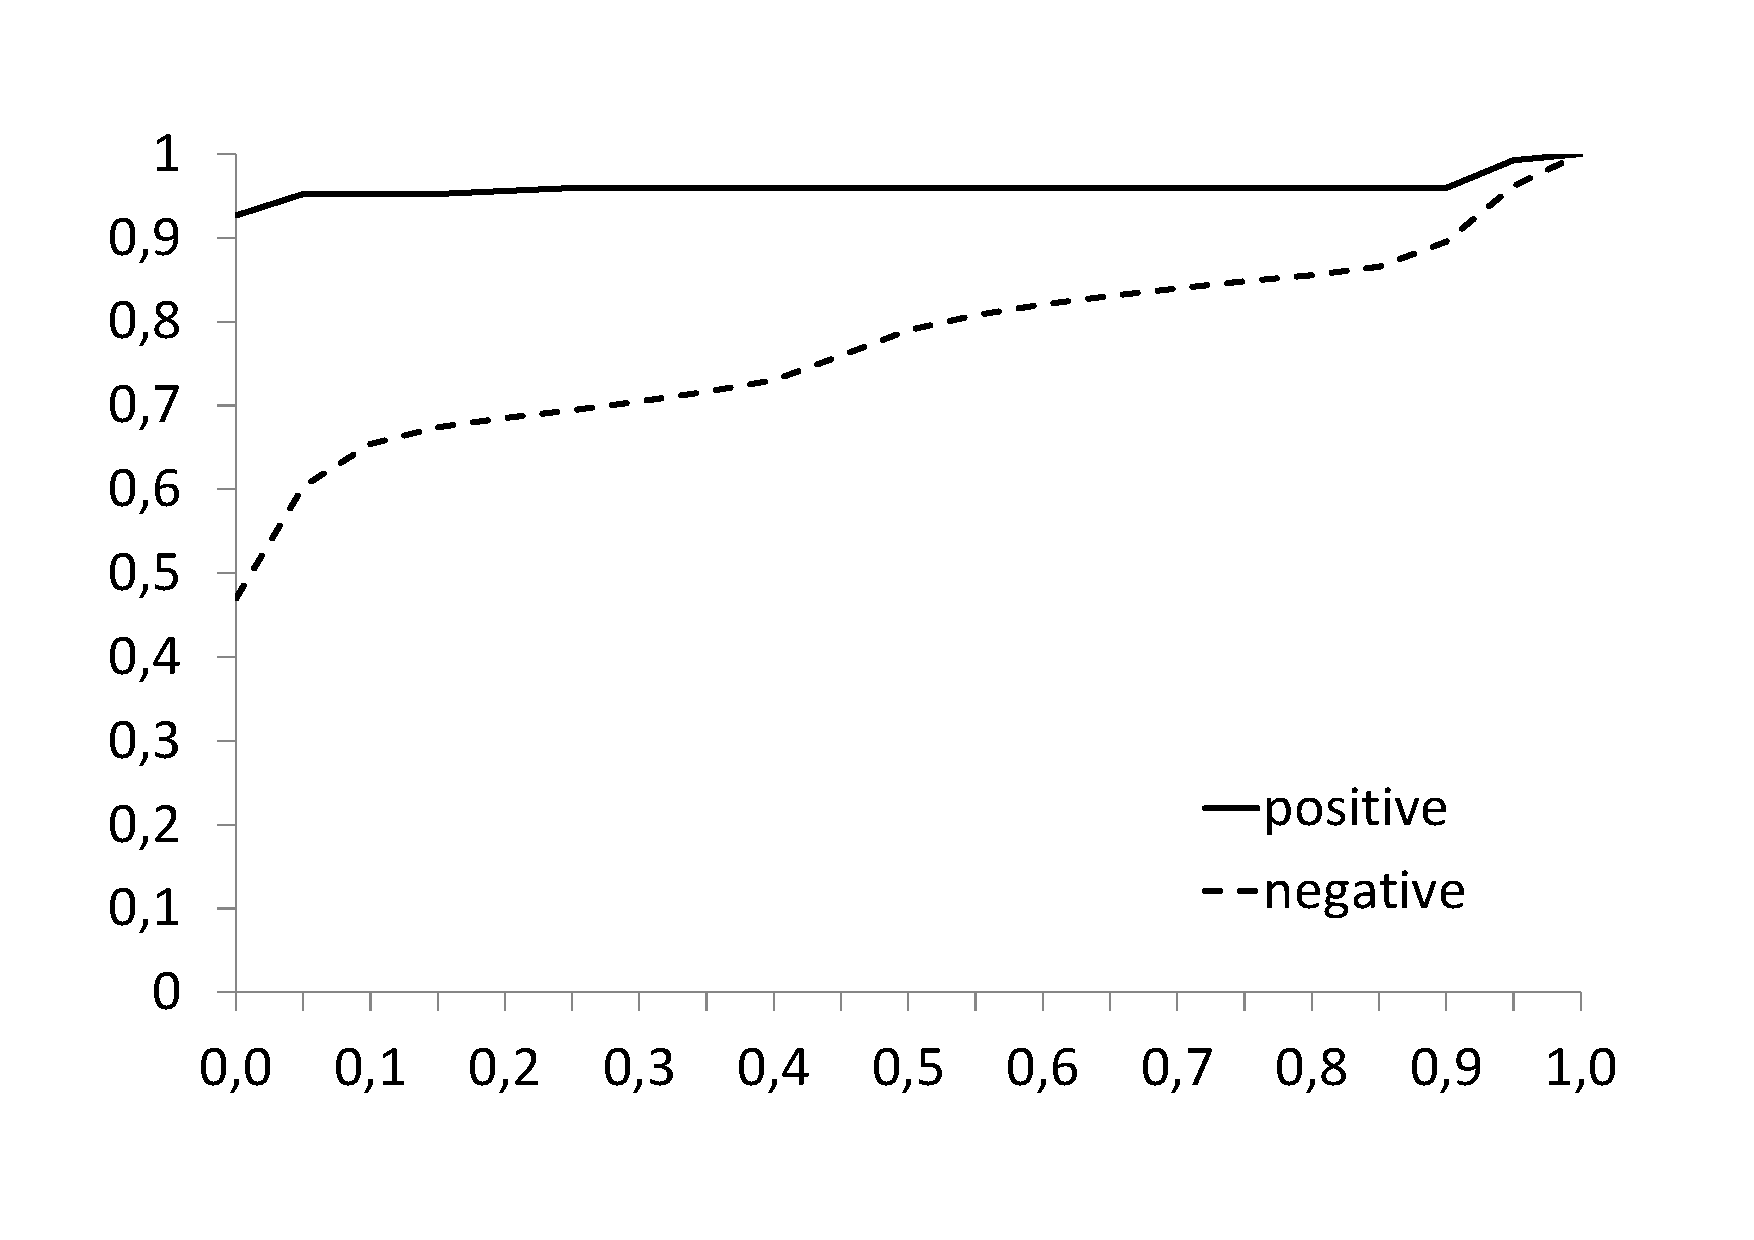
\includegraphics[height=4.1cm]{grafsyn2all.pdf} }}%
    \qquad
    \subfloat[RST / ALL]{\label{fig:grafrst2all}{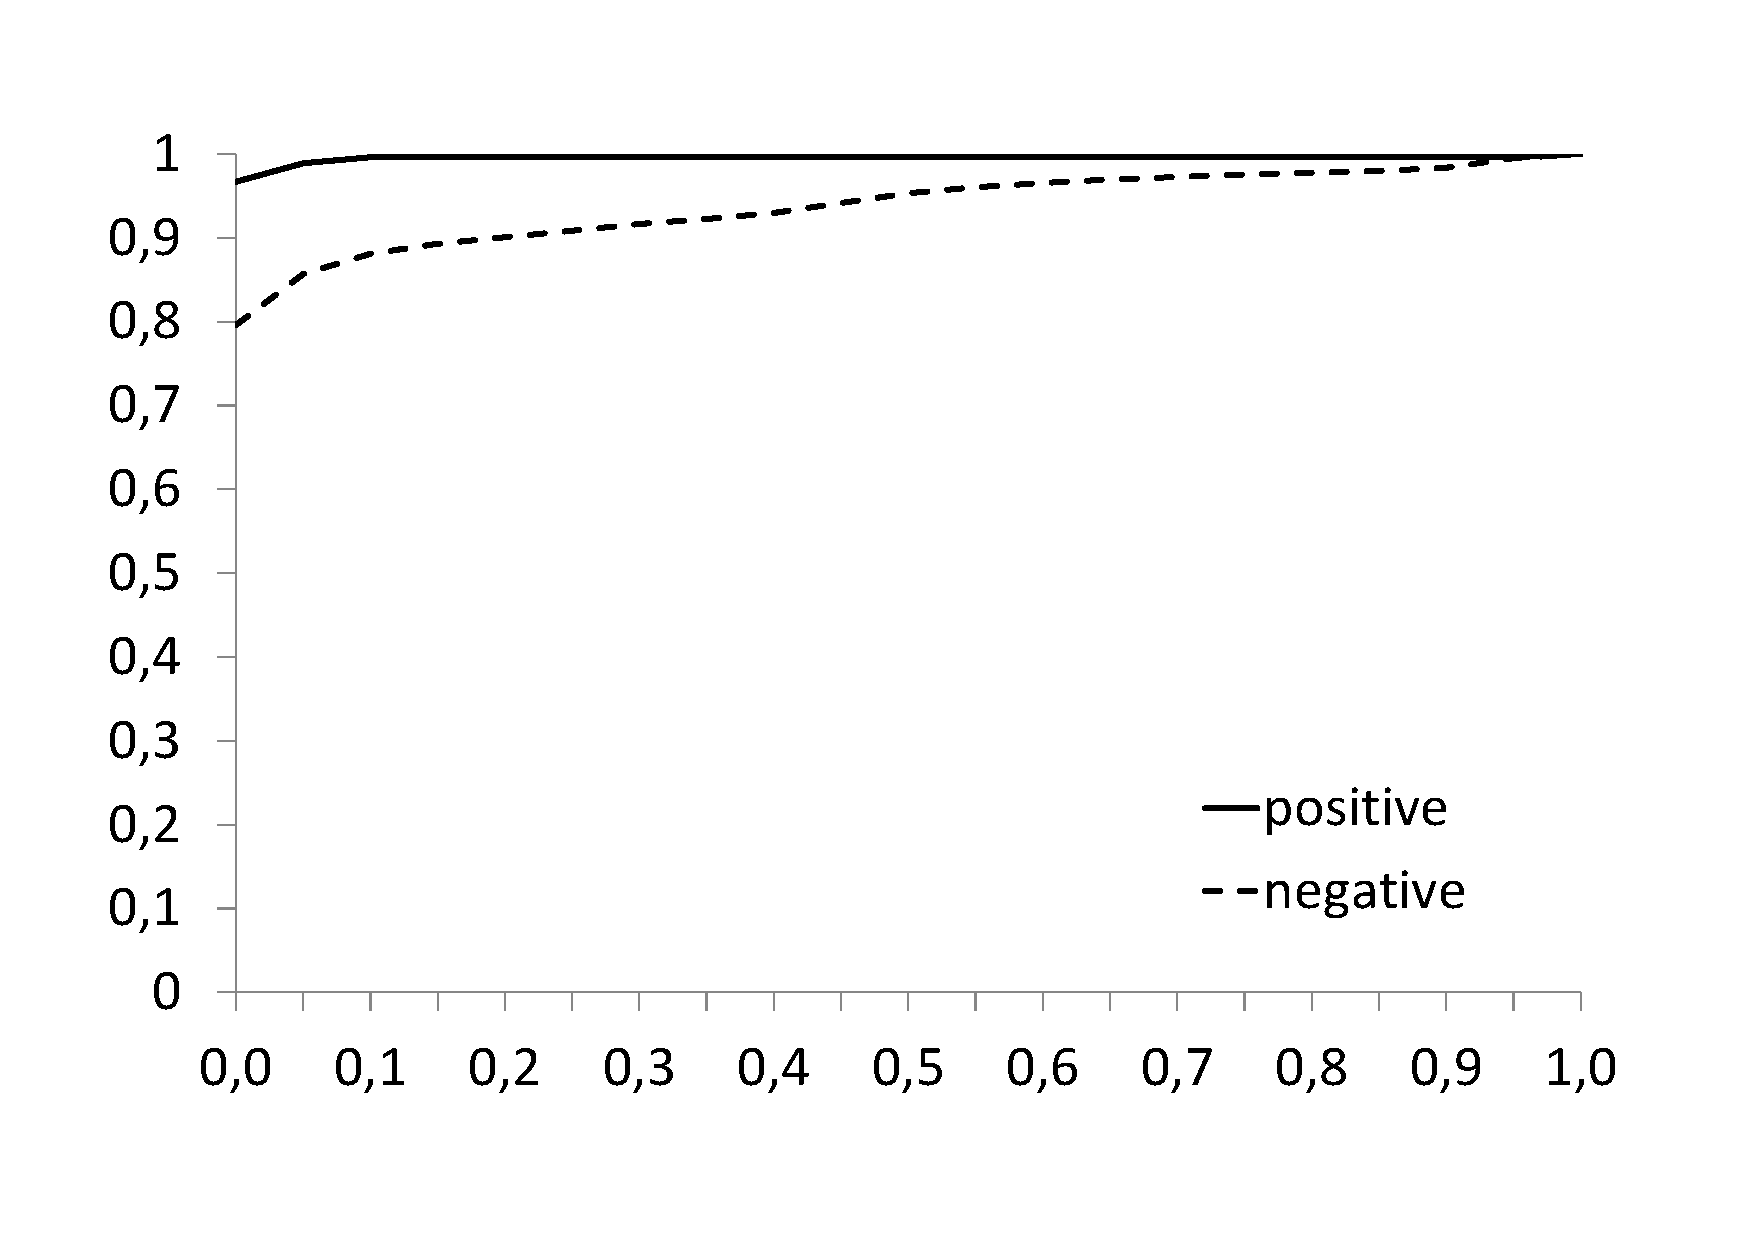
\includegraphics[height=4.1cm]{grafrst2all.pdf} }}\\
    \subfloat[FIN / ALL]{\label{fig:graffin2all}{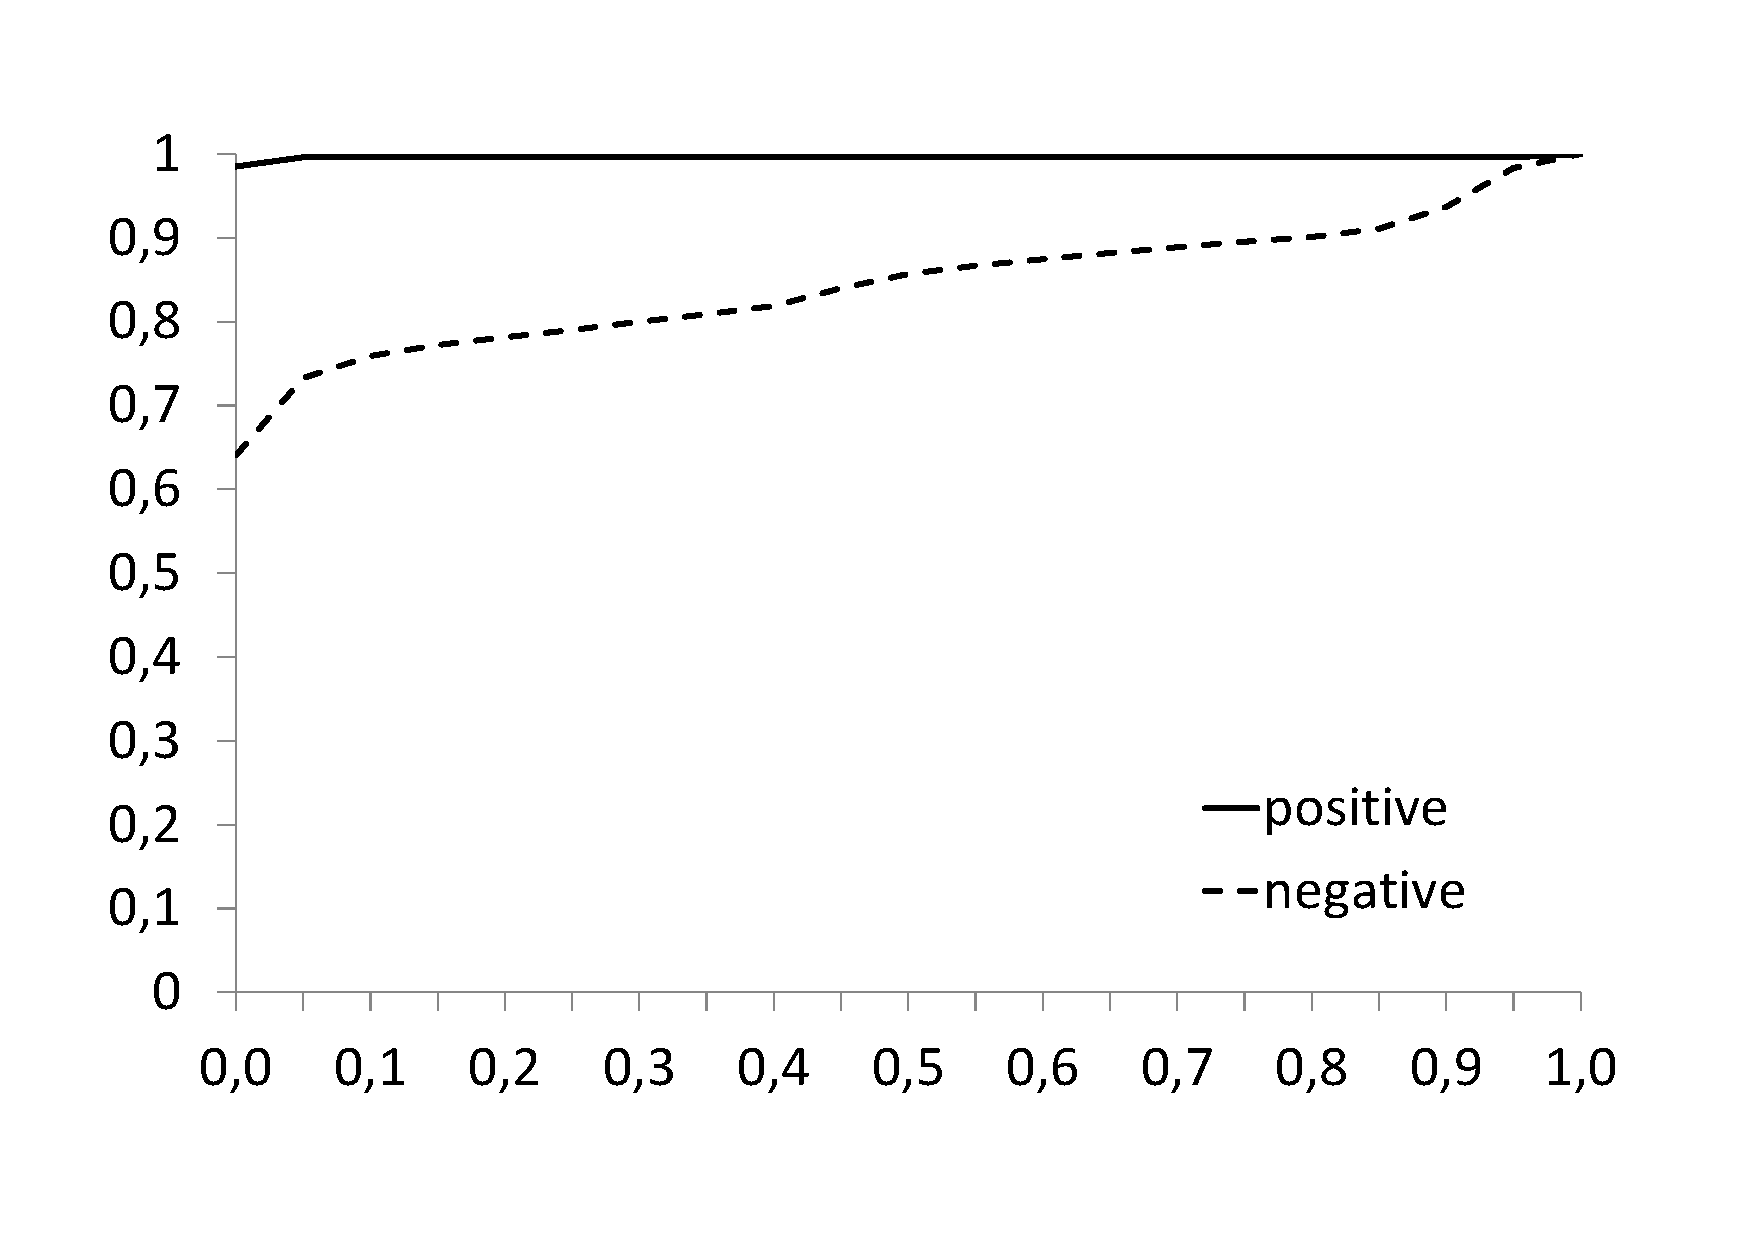
\includegraphics[height=4.1cm]{graffin2all.pdf} }}%
   % \qquad
    %\subfloat[reqest to all]{\label{fig:grafreq2all}{\includegraphics[height=4.1cm]{grafreq2all.pdf} }}%
    \caption{Cumulative distribution function of features}%
    \label{fig:histograms}%
\end{figure}

In Figure~\ref{fig:grafbpp} we can observe that the distribution of positives and negatives differs significantly.
Please note that the x-axis of this figure was shortened to display the detail.
More than 50\% of positives accounts for packets of size 105 to 110 bytes, and another 40\% accounts for packets of average size from 35 to 80 bytes. 
On the other hand, 20\% of negative triplets consists of packets of a size smaller than 35 bytes, another 20\% accounts for packets of size 80 to 105 bytes, and another 20\% accounts for packets larger than 110 bytes.

Distribution of a number of packets per flow (in Figure~\ref{fig:graflogppf}) and packets per minute (in Figure~\ref{fig:graflogppm}) are correlated. 
Positive triplets belong to either a weak group with a low number of packets or a strong group with a high number of packets per flow as well as per minute.
Moreover, in the case of negative triplets there exists less than 1\% of instances with an extremely high number of packets.

Figure~\ref{fig:grafackpush} displays the distribution of the rate of flows with push and ack flag set to all flows.
The CDF of negatives shows that there is more than 20\% of triplets without any ack and push flags set. 
The CDF of negatives slowly rises to 40\% at the rate of 0.8. 
On the other hand, there are nearly zero positives with a rate lower than 0.8 while the majority of positives exhibits rate higher than 0.9.
The opposite holds for distribution of other flags depicted in Figures~\ref{fig:grafsyn2all},~\ref{fig:grafrst2all},~\ref{fig:graffin2all}. 
Positives with zero rate account for the majority of its samples while negatives only for 50\% in case of SYN, for 80\% in case of RST and 65\% in case of FIN.

Last but not least, the detection works upon requests from miners to the mining server. To this end, the feature capturing the rate between the number of flows with source port greater than destination port to all the flows aims at distinguishing between a prevalent request or response communication. By keeping the rate as one of the features and not an a priori condition we allow the detection algorithm to detect miners even in those triplets that aggregate responses if the other features recognize that triplet as potentially positive. This makes the algorithm more robust but for the price of more false positives and the higher number of triplets to work with. The distribution of positives as well as of negatives are almost identical.% (Figure~\ref{fig:grafreq2all}).
 
Obviously, none of the features considered is good enough to directly distinguish between positives and negatives. Therefore, the detection algorithm must combine results of several features to improve detection results.

We evaluate two detection algorithms, one designed manually and one based on machine learning, both described in Section~\ref{subsec41}.

As the training and evaluation data-set contains a significantly lower number of mining communications (273 positive triplets) than of other communications (356,574 negative triplets), we apply {\it ClassBalancer} filter to balance the weight of both sets in order not to overtrain the detector on non-mining communications.
The training process is set up with the following parameters 5-fold cross-validation, and the number of instances in a leaf must be at least 100 (other parameters are kept default).

The higher number of instances in a leaf, the less deeper tree is generated by the training process. And the less deeper tree, the faster is its evaluation as well as the tree is less overfitted to a particular data-set.

The confusion matrix of the resulting detector is depicted in Table~\ref{tab:conf1}. It shows ML-detector marks: a) mining communication as mining in most cases; b) another communication as other; c) except in 2.6\% of cases where communication is misclassified as mining (i.e., false positive); and d) although the ML-detector misclassifies 4.7\% of mining triplets, it is a significant improvement over the manually constructed classifier. 

\begin{table}[htp]
    \begin{center}
        \begin{tabular}{|c|c|c|}
            \hline
            Classified as & other & mining \\
            \hline
            other   & 97.4\% & 2.6\% \\
            mining  & 4.7\% & 95.3\% \\
            \hline
        \end{tabular}
    \caption{Confusion matrix of classified triplets by the decision tree.}
    \label{tab:conf1}
    \end{center}
\end{table}

\begin{table}[htp]
 \begin{center}
\begin{tabular}{|c|c|c|}
 \hline
 Classified as & other & mining \\
 \hline
other   & 91.4\% & 8.6\% \\
mining  & 10.3\% & 89.7\% \\
 \hline
 \end{tabular}
 \caption{Confusion matrix of classified triplets by the manual classifier.}
 \label{tab:conf2}
 \end{center}
\end{table}

The confusion matrix of the manual classifier is depicted in Table~\ref{tab:conf2}.

Although the manual classifier was utilized to collect the annotated training and evaluation data-set, it fails to correctly classify approx. 10\% of each class.
This discrepancy is caused by the mining servers list which is gradually built whenever passive detection is successful.
Once this list is populated, the manual classifier also identifies such mining triplets that would otherwise not meet enough conditions of the classifier.

%%%%%%%%%%%%%%%%%%%%%%%%%%%%%%%%%%%%%%%%%%%%%%%%%%%%%%%%%%%%%%
%Vyhodnoceni detektoru
%%Vyhodnoceni rychlosti konvergence
%The detection generates many false positives which are reduced by the verification probe or by the list of verified servers. Before the list is built the number of probes per second would be too high due to the high number of unique triplets appearing, approximately 4000/s unique triplets in our data-set at the beginning. While the list is built it becomes 
%%Testovanie prebiehalo na sieti CESNET s obmedzením na 3 podsiete:
%%147.229.0.0/16 - podsieť VUT
%%147.231.0.0/16 - podsieť AVČR
%%147.251.0.0/16 - podsieť MUNI
%%Počet unikátnych trojic za sekundu je približne 4000 (presne 3900). Údaj je priemerom meraní z %%troch dní v čase od 6. hodiny ráno do 22. hodiny večer.
%%Veľkosť fasthash table bola odvodená na základe počtu unikátnych trojíc za sekundu tak, aby sa %%predišlo vyhadzovaniu položiek z tejto tabulky. Veľkost pre testovanie bola nastavená na 8388608 %%(2 power 23) riadkov, pričom jeden riadok obsahuje 4 položky.
%%pocet detekci bez aktivniho testu pri zmene tresholdu
%%co se nejcasteji detekuje jako falesne pozitivni
%%pocet aktivnich testu behem casu
%%%%%%%%%%%%%%%%%%%%%%%%%%%%%%%%%%%%%%%%%%%%%%%%%%%%%%%%%%%%%%


%% ===========================================================

\section{Catalog of Mining Pools}
\label{sec5}
We were also looking for a more lightweight solution suitable even for small corporate networks lacking capacities to install dedicated probes performing our active/passive traffic monitoring employing machine learning. We want to offer conclusive detection results with a minimum set of input information. 

Network administrator and law enforcement agent (i.e., our main actors for mining detection use-case) shall have basic NetFlow records of investigated device/network segment. These records contain at least source/destination IP addresses, source/destination ports and a protocol identifier. The reasoning behind our second approach is following. If we know IP address of mining pool server, then we can reliably distinguish between mining and non-mining connections. Moreover, if we are aware of the port number employed by a pool operator, then we can tell what cryptocurrency is being mined through the connection. 

\subsection{Design}
\label{subsec51}
Both mining server's hostname and port number are publicly available (except mining malware cases) on pool's webpage because they are necessary for successful setup of the mining process. Without this vital information, the miner would not be able to configure mining software properly.

Based on these premises, we have decided to manually collect all mining software configurations announced by the biggest mining pools for several important cryptocurrencies. We gathered all these data in a database, which is accessible through a web application called sMaSheD (Mining Server Detector of cryptocurrency pools). In the rest of this subsection, we briefly outline some of the design choices that we have made during the sMaSheD development.

%Vyber kryptomen
There are hundreds of coins (and tokens) available in cryptocurrency universe. In order to choose coins supported by sMaSheD, we did due diligence on "the most popular" cryptocurrencies taking into account public news \cite{BLOOMBERG}, dedicated reports \cite{CARBON-BLACK} and consultations with our LEA partners. Bitcoin is dominating this ladder due to its importance (e.g., around 80 million USD worth of Bitcoins stolen from a hacked cloud mining service provider in December 2017 \cite{REDDIT-NICEHASH}). However, Monero becomes more and more used by malwares because of its anti-forensic features, which help to cover criminal's tracks (e.g., nearly 5\% of all Moneros in circulation worth of 175 million USD were mined using malware \cite{PALOALTO-MONERO}). The third is Ethereum thanks to smart-contracts and popularity among token developers (e.g., 30 million USD worth of Ethereum stolen by a wallet breach in July 2017 \cite{COINDESK-ETHERSTEAL}). No matter on the current set of cryptocurrencies, sMaSheD is designed to be a generic catalog of mining pools which should be easy to maintain and operate.

%Vyber poolu
As a next step, we investigated mining distribution among available pools for each chosen cryptocurrency. The majority of pools add their signature into the freshly mined block. This marking allows to account the success rate of each participating pool. Moreover, pools are announcing their overall hashrate performance publicly. By combining these data, we receive quite a reliable overview about more and less important pools for every cryptocurrency. Anyone can obtain these data from dedicated web-pages, e.g. \cite{BLOCKCHAININFO-POOLS} for Bitcoins, \cite{LITECOIN-POOLS} for Litecoin, and \cite{ETHERSCAN-POOLS} for Ethereum. 

Mining software configurations are collected by web scraping the content of pool web pages. This procedure is currently performed manually by sMaSheD administrators. However, we aim at the automation of this process in the near future. The following set of information is being collected for every pool (from web-pages similar to \ref{appendix-sec1}):

\begin{itemize}
    \item the name of the pool and its home URL;
    \item the list of pool servers identified by FQDN including ports associated with a mined cryptocurrencies;
    \item every mining server FQDN is resolved onto a list of IPv4/IPv6 addresses.
\end{itemize}

Nevertheless, some pools are private (e.g., Bitfury pool with roughly 2\% hashrate share \cite{BTCCOM-BITFURY} run by a company\footnote{For more, visit https://bitfury.com/} with the same name producing ASIC mining solutions). The operator of such pool does not maintain any publicly available web page, which makes any web scraping of configuration impossible. Hence, sMaSheD catalog does not contain a complete list of pools for a given cryptocurrency. Fortunately, private pools constitute a fraction of overall network hashrate.

%Resolving DNS
Mining server FQDNs may include information about location, mined cryptocurrency (e.g., \texttt{eth-us2.dwarfpool.com}) or employed algorithm (e.g., \texttt{sha256.eu.nicehash.com}). However, a single visit of a pool's web page does not take into account the changing nature of pool infrastructure (i.e., mining service availability on new/old servers). Thus, we conducted experiments with automated discovery of FQDNs. We tried to generate hostnames as permutations from a set of keywords, which includes cryptocurrency abbreviations, country codes and pool domains. Unfortunately, this approach: 1) generated way too many false hostnames; and 2) verification of generated hostnames is a time consuming process. DNS allows listing of all records (including hostname A and AAAA records) through zone transfer\footnote{For more about DNS records and zones, please read RFC 1035 and related ones.}, but this is not applicable for our use-case.

Pool operators provide a server FQDNs, which are resolved by miners onto various IP address based on miner's geolocation. Based on deployment (see Figure \ref{fig:deploy}), DNS may resolve a single FQDN onto many IP address (e.g., \texttt{stratum.slushpool.com}) in order to guarantee high-availability of mining service. sMaSheD tries to keep the list of these IP addresses as up-to-date as possible. It is a necessity especially for pools leveraging cloud deployment because cloud providers often rotate available IP addresses among customers' virtual machines. An IP address of mining server today can belong to a completely different machine tomorrow. Because of this changing nature and since a single FQDN may actually represent a set of load-balancing mining servers, sMaSheD periodically renews the list of IP addresses associated with each mining server within the system.

In order to provide more reliable results if a given IP address belongs to a mining server or not, we developed probing similar to one described in Section \ref{sec4}. This probing repeats for all known pools (and their mining servers) every 3 hours as a background task asynchronous to web application run. During every periodic check of mining server, sMaSheD sends crafted mining protocol message and waits for the response. If counterparty reacts properly (with a message containing work package), then it confirms that this device is really a pool's mining server.

%Probing
Probing is supported for Stratum and GetBlockTemplate mining protocols. sMaSheD is probing single server for both of these protocols. GetWork is also implemented, but we were not able to test it since this protocol is deprecated and not employed by any pool within our system. There are three probing return codes:

\begin{itemize}
    \item DOWN - Probing failed because connection had not been even established. This occurs when a port on the server is closed, or some middle-box is blocking the connection.
    \item LISTEN - The connection was accepted on a specified port, but the alleged server returns an empty response. This happens when a) server is using different mining protocol than tested one; b) port is opened but bound to a different application.
    \item UP - Probing succeeded because mining server responded with mining protocol message containing valid content. Message validity depends on employed mining protocol and consists of multiple value presence tests (e.g., \textit{error}, \textit{result} and other JSON fields). This validator can be easily extended to support changes or even new mining protocols.
\end{itemize}

Probing return code is usually accompanied with a verbose result (i.e., destination unreachable, unknown method, mining subscribe). sMaSheD records each probing attempt, which creates a history of service availability for a given mining server. These temporal data can later prove that IP address was used by a mining server (at least from the perspective of sMaSheD).

\subsection{Evaluation}
\label{subsec52}
In order to validate probing results, we compared the behavior of sMaSheD with official mining software. We decided to use cgminer 3.7.2 \cite{CGMINER} because it is well-established and supports all available mining protocols. 

We tested both tools over the same set of mining servers and recorded communication into PCAP file. We compared connection success rate (based on textual console outputs) and messages exchanged between miner (either sMaSheD or cgminer) and mining server. We did not find any differences for detected mining servers when comparing sMaSheD and cgminer connection attempts. Both applications used the same set (1983 entries) of IP addresses and ports of alleged mining servers. 

sMaSheD system does not send any authentication credentials towards a pool upon the check, the basic response for mining subscription message is enough to mark a device as mining server positively. This is illustrated in Wireshark message captures depicted in Figure \ref{fig:wshark-cgminer} and Figure \ref{fig:wshark-smashed}.

sMaSheD is coded as a web application employing PHP framework Laravel 5.6 with front-end based on Bootstrap 3. The system is operated in a Docker container on CentOS 7. All source codes are available on \cite{GITHUB-SMASHED}. 

Figure in \ref{appendix-sec2} explains relations between data available in the system. All data can be easily obtained in JSON via REST API. The database of sMaSheD currently (in August 2018) contains:

\begin{itemize}
    \item 13 cryptocurrencies mined on 18 various port numbers;
    \item 56 pools operating 184 servers with 479 addresses;
    \item 2284 probing associations (dubbed as mining properties) and it takes approximately 20 minutes to them (i.e., check all IP-port tuples of all known mining servers for both Stratum and GetBlockTemplate).
\end{itemize}

Mining pools catalog sMaSheD (implemented as the second approach solution for miners detection):

\begin{itemize}
    \item offers access to all data in JSON format through REST calls;
    \item periodically probes available pools' servers whether they provide mining services and accounts the result;
    \item allows privileged users to update database according to the current situation (i.e., add newly established pools).
\end{itemize}

\begin{figure}[tp]
    \centering
    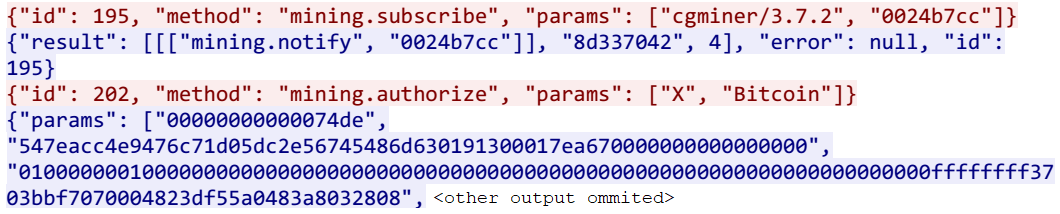
\includegraphics[width=\textwidth]{wshark-cgminer.png}
    \caption{Message exchange between cgminer (red) and pool (blue)}
    \label{fig:wshark-cgminer}
\end{figure}

\begin{figure}[tp]
    \centering
    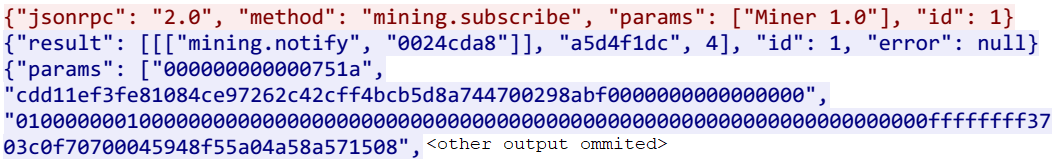
\includegraphics[width=\textwidth]{wshark-smashed.png}
    \caption{Message exchange between sMaSheD (red) and pool (blue)}
    \label{fig:wshark-smashed}
\end{figure}

%% ===========================================================

\section{Conclusion}
\label{sec6}

%% Prinosy
In this paper, we provided an in-depth analysis of cryptocurrency mining operation. We designed and implemented sMaSheD catalog and passive-active detection approaches to detect mining devices within the network. We tested the feasibility of these approaches on real-life data as well as published data-sets utilized in this article under open access policy. We conclude that catalog and passive-active approach are complementary. 

%% Zhodnoceni detekce
The results of passive-active detection approach show that although there is a high number of false positives after the passive detection, it is sufficiently low to enable active verification of the results. In comparison to the pure catalog approach, passive-active detection is capable of discovering emerging or deliberately hidden pools. As such it should serve Security Operation Centers, CSIRT, and network security service providers to populate their cyber threat intelligence systems.

%% Zhodnoceni katalogu
The goal of our sMaSheD system is to become a tool as valuable for network administrators and LEA operatives as what is ExoneraTor \cite{EXONERA} application for TOR overlay network. sMaSheD prototype including a large data-set is available at \cite{WWW-SMASHED} (see \ref{appendix-sec3} for demo screenshots). Moreover, anyone can deploy own installation from sources \cite{GITHUB-SMASHED} and feed it with custom pools. Online catalog offers a curated list of the most popular pools and their servers. Data available in sMaSheD offer a neat solution for following use-cases:

\begin{itemize}
    \item create an access control list that will block unwanted traffic mining traffic (based on IPs and ports known to sMaSheD);
    \item detect the presence of miners via inspection of their DNS queries (based on FQDNs and IPs contained in DNS requests and answers);
    \item data-retention proof about mining service availability for a given IP+port tuple.
\end{itemize}

%% Budoucnost
We would like to automatize metadata collection for sMaSheD by a periodic scraping of relevant web pages. Currently, the information provided by our catalog is updated manually, which makes the system less dynamic than we would appreciate. Regarding additional future work, we also consider other strategies on how to probe and positively identify pool servers based on different mining protocol messages. Last but not least, we are constantly adding new cryptocurrencies, pools, and servers as they appear in publicly disclosed announcements of illicit mining activities. 

%%Acknowledgement
This article has been supported by the Ministry of Education, Youth and Sports from the National Programme of Sustainability (NPU II) project IT4Innovations excellence in science (no.  LQ1602). 
Authors also want to acknowledge work done by Jakub Kelečeni, Erik Šabík, and Martin Cagaš, the students of Brno University of Technology.

%% References
%%
%% Following citation commands can be used in the body text:
%% Usage of \cite is as follows:
%%   \cite{key}         ==>>  [#]
%%   \cite[chap. 2]{key} ==>> [#, chap. 2]
%%

%% References with bibTeX database:

\bibliographystyle{elsarticle-num}
% \bibliographystyle{elsarticle-harv}
% \bibliographystyle{elsarticle-num-names}
% \bibliographystyle{model1a-num-names}
% \bibliographystyle{model1b-num-names}
% \bibliographystyle{model1c-num-names}
% \bibliographystyle{model1-num-names}
% \bibliographystyle{model2-names}
% \bibliographystyle{model3a-num-names}
% \bibliographystyle{model3-num-names}
% \bibliographystyle{model4-names}
% \bibliographystyle{model5-names}
% \bibliographystyle{model6-num-names}

\bibliography{sample}


\pagebreak
%% The Appendices part is started with the command \appendix;
%% appendix sections are then done as normal sections
\appendix

\section{Mining software configuration}
\label{appendix-sec1}

\begin{figure}[!hb]
    \centering
    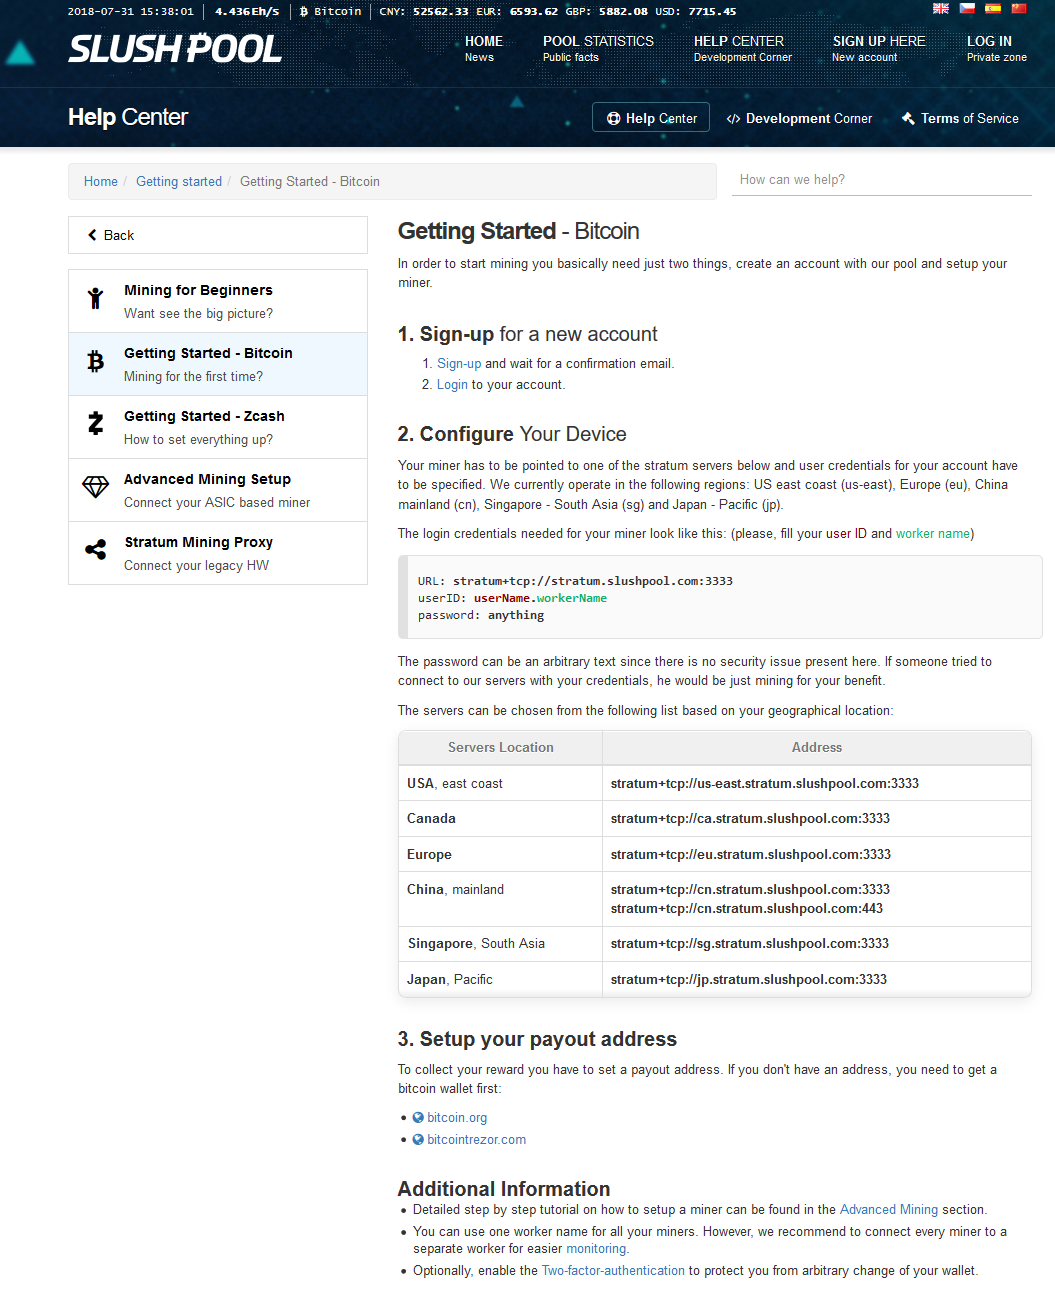
\includegraphics[width=0.95\textwidth]{slushpoolconfig.png}
    \caption{Example of mining software setup taken from SlushPool}
    \label{fig:slushpool}
\end{figure}

\section{E-R Diagram}
\label{appendix-sec2}

\begin{figure}[!hb]
    \centering
    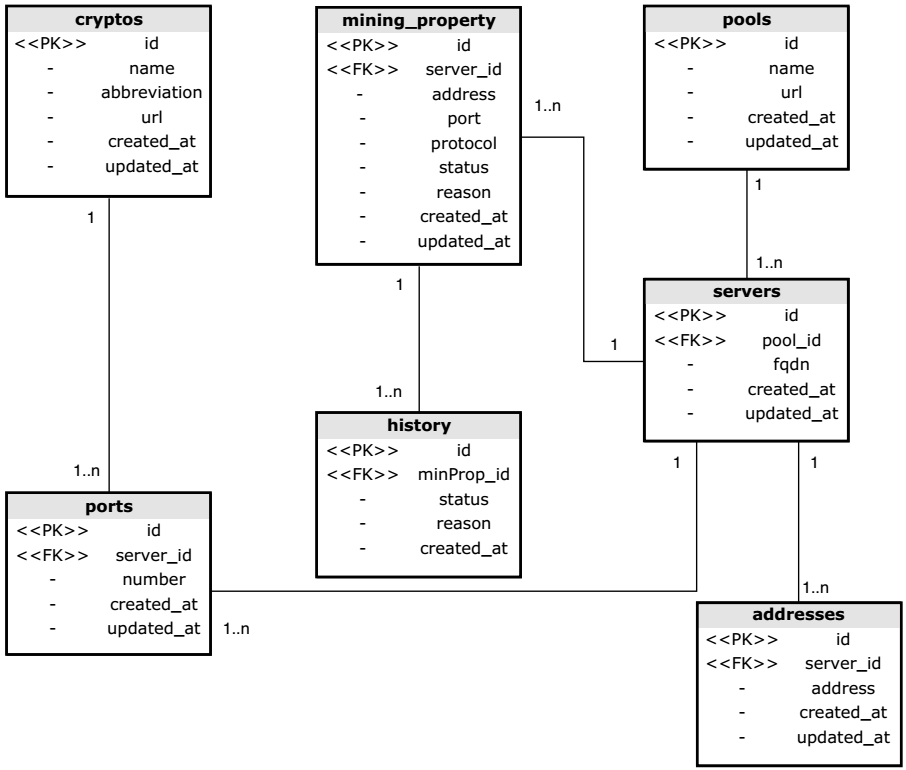
\includegraphics[width=\textwidth]{erdiag.png}
    \caption{Entity Relationship diagram for sMaSheD database}
    \label{fig:erdiagram}
\end{figure}

\pagebreak
\section{sMaSheD Demo}
\label{appendix-sec3}

\begin{figure}[!h]
    \centering
    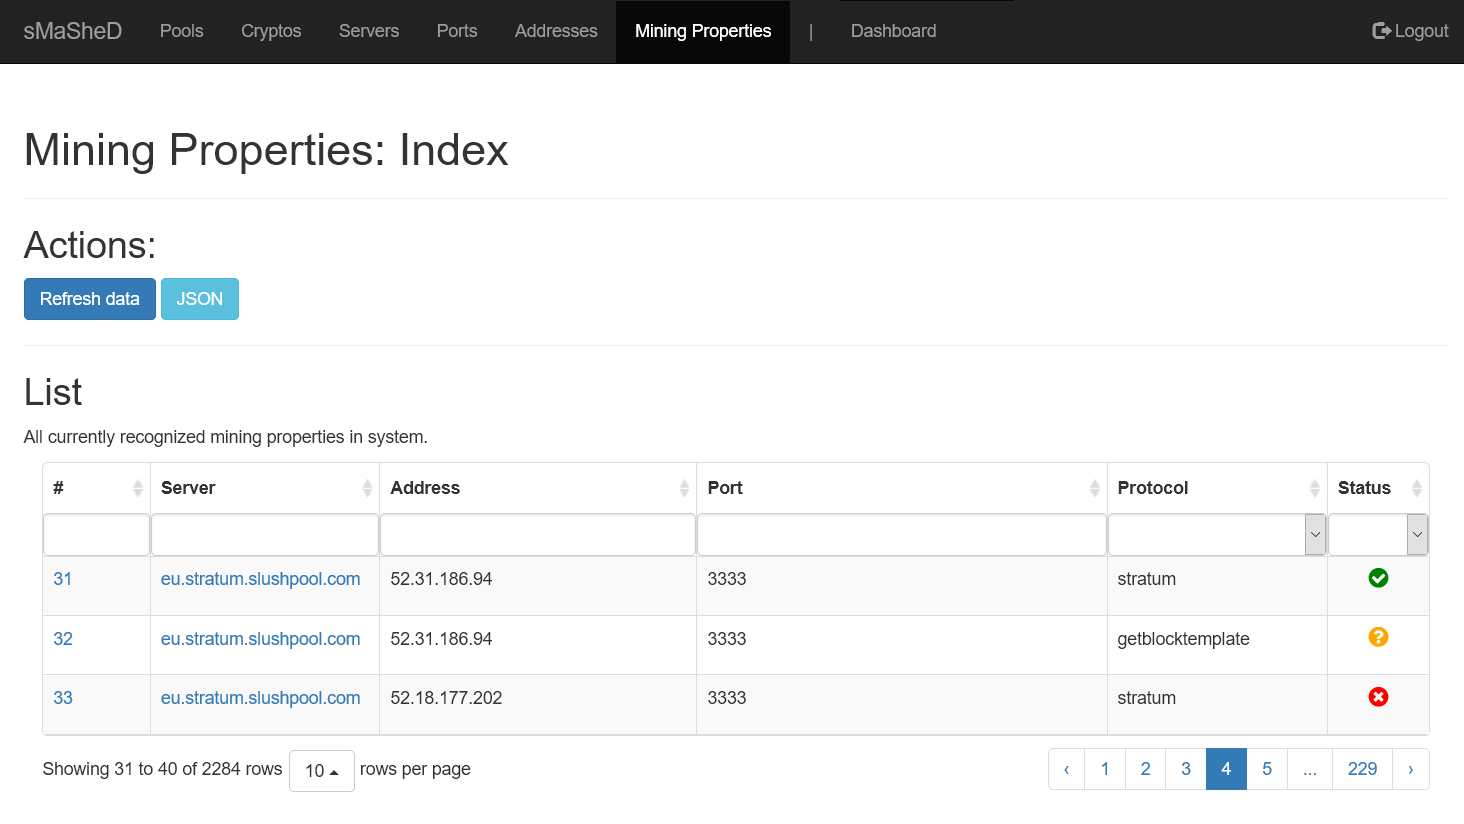
\includegraphics[width=0.9\textwidth]{smashed1.png}
    \caption{Probe results of selected subset from all available mining servers}
    \label{fig:smashed1}
\end{figure}

\begin{figure}[!h]
    \centering
    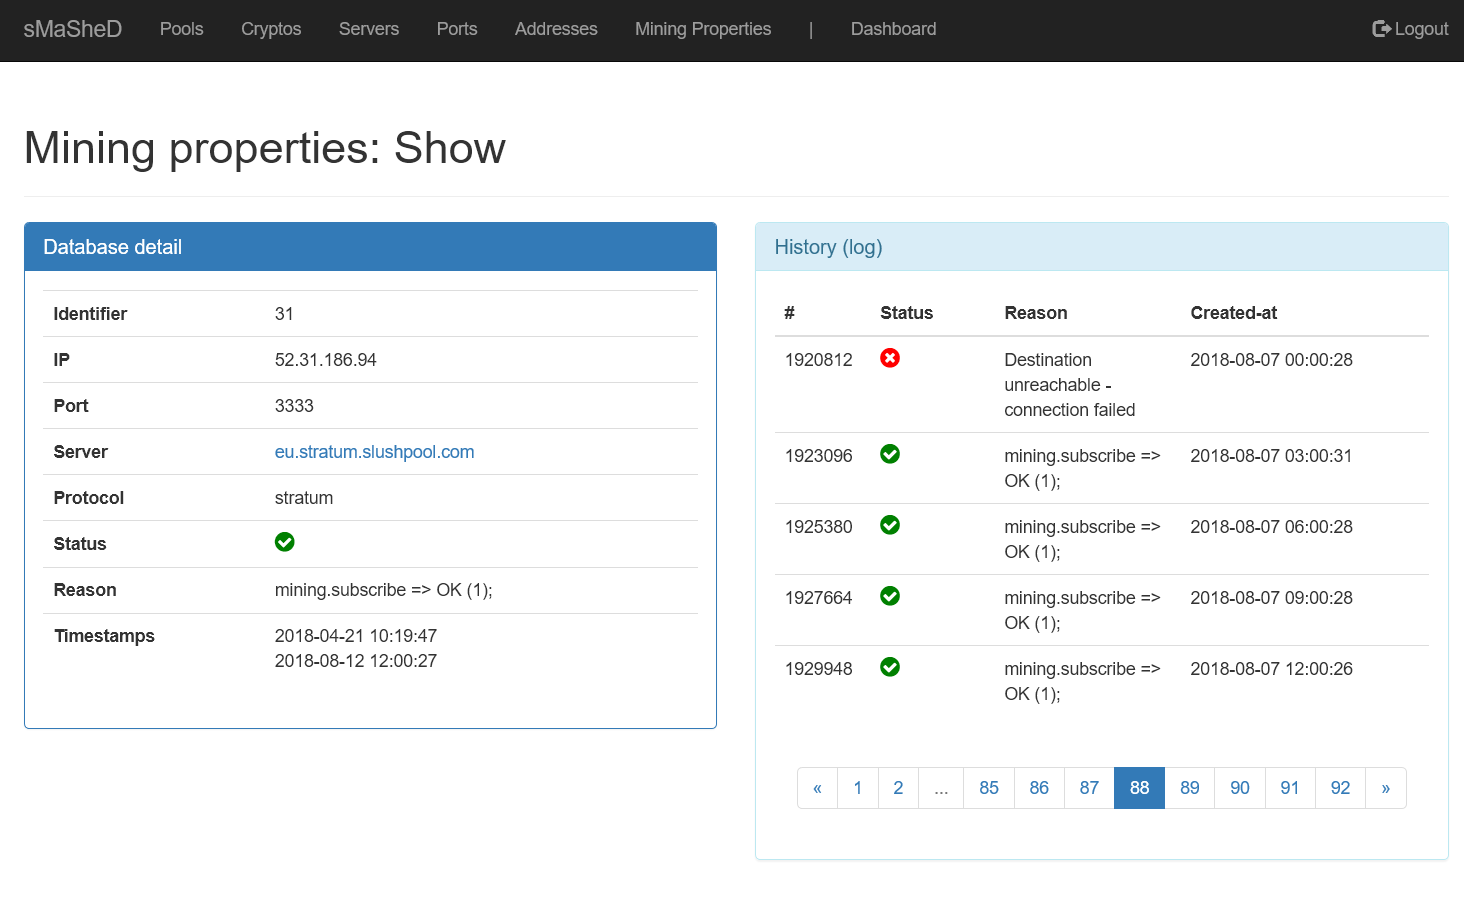
\includegraphics[width=0.9\textwidth]{smashed2.png}
    \caption{Log of probe attempts for a given mining server}
    \label{fig:smashed2}
\end{figure}


\end{document}

%%
%% End of file `elsarticle-template-num.tex'.


%%%%%%%%%%%%%%%%%%%%%%%%%%%%%%%%%%%%%%%%%%%%%%%%%%%%%%%%%%%%%%
% === Run information ===
% 
% Scheme:       weka.classifiers.trees.J48 -C 0.9 -M 400
% Relation:     weka_train-weka.filters.supervised.instance.ClassBalancer-num-intervals10
% Instances:    100273
% Attributes:   9
              % ackpush/all
              % bpp
              % ppf
              % ppm
              % req/all
              % syn/all
              % rst/all
              % fin/all
              % class
% Test mode:    10-fold cross-validation
% Evaluation cost matrix:
   % 0   1
 % 100   1
% 
% 
% === Classifier model (full training set) ===
% 
% J48 pruned tree
% ------------------
% 
% ppm <= 135
% |   bpp <= 70
% |   |   ppm <= 12
% |   |   |   rst/all <= 1
% |   |   |   |   fin/all <= 7
% |   |   |   |   |   ppf <= 3
% |   |   |   |   |   |   bpp <= 59
% |   |   |   |   |   |   |   ackpush/all <= 86: notminer (147.4)
% |   |   |   |   |   |   |   ackpush/all > 86
% |   |   |   |   |   |   |   |   ppf <= 1
% |   |   |   |   |   |   |   |   |   ppm <= 3: miner (3009.45/254.69)
% |   |   |   |   |   |   |   |   |   ppm > 3: notminer (543.13/183.65)
% |   |   |   |   |   |   |   |   ppf > 1
% |   |   |   |   |   |   |   |   |   ackpush/all <= 99
% |   |   |   |   |   |   |   |   |   |   ackpush/all <= 98: miner (11605.76/403.1)
% |   |   |   |   |   |   |   |   |   |   ackpush/all > 98: notminer (49.13)
% |   |   |   |   |   |   |   |   |   ackpush/all > 99: miner (4648.41/57.16)
% |   |   |   |   |   |   bpp > 59
% |   |   |   |   |   |   |   syn/all <= 94
% |   |   |   |   |   |   |   |   ackpush/all <= 99: notminer (1381.26)
% |   |   |   |   |   |   |   |   ackpush/all > 99: miner (607.1/56.15)
% |   |   |   |   |   |   |   syn/all > 94: miner (1876.61/40.11)
% |   |   |   |   |   ppf > 3
% |   |   |   |   |   |   ackpush/all <= 99: notminer (882.4)
% |   |   |   |   |   |   ackpush/all > 99: miner (934.14/199.54)
% |   |   |   |   fin/all > 7: notminer (857.84)
% |   |   |   rst/all > 1
% |   |   |   |   ppf <= 5: notminer (2058.6)
% |   |   |   |   ppf > 5
% |   |   |   |   |   rst/all <= 15: miner (400.89/33.59)
% |   |   |   |   |   rst/all > 15: notminer (609.66)
% |   |   ppm > 12: notminer (4073.59)
% |   bpp > 70
% |   |   ppm <= 70
% |   |   |   req/all <= 75: miner (367.3)
% |   |   |   req/all > 75: notminer (37866.59)
% |   |   ppm > 70: miner (1467.55/182.0)
% ppm > 135
% |   bpp <= 103: notminer (530.95)
% |   bpp > 103
% |   |   bpp <= 108: miner (26279.52/17.55)
% |   |   bpp > 108: notminer (75.71)
% 
% Number of Leaves  : 	22
% 
% Size of the tree : 	43
% 
% 
% Time taken to build model: 1.85 seconds
% 
% === Stratified cross-validation ===
% === Summary ===
% 
% Correctly Classified Instances       96578.4891          96.3155 %
% Incorrectly Classified Instances      3694.5109           3.6845 %
% Kappa statistic                          0.9263
% Total Cost                          287801.3443
% Average Cost                             2.8702
% Mean absolute error                      0.0483
% Root mean squared error                  0.1827
% Relative absolute error                  9.6521 %
% Root relative squared error             36.5374 %
% Coverage of cases (0.95 level)          97.7771 %
% Total Number of Instances           100273     
% 
% === Detailed Accuracy By Class ===
% 
                 % TP Rate  FP Rate  Precision  Recall   F-Measure  MCC      ROC Area  PRC Area  Class
                 % 0,974    0,048    0,953      0,974    0,964      0,927    0,977     0,961     notminer
                 % 0,952    0,026    0,973      0,952    0,963      0,927    0,977     0,978     miner
% % Weighted Avg.    0,963    0,037    0,963      0,963    0,963      0,927    0,977     0,969     
% 
% % === Confusion Matrix ===
% 
     % a        b      <-- classified as
 % 48829.44  1307.06 |        a = notminer
  % 2387.45 47749.05 |        b = miner
%%%%%%%%%%%%%%%%%%%%%%%%%%%%%%%%%%%%%%%%%%%%%%%%%%%%%%%%%%%%%%
